\documentclass[11pt]{article}
\usepackage[T1]{fontenc}
\usepackage[a4paper,margin=26mm]{geometry}
\usepackage{amsmath,amssymb,amsthm,mathtools}
\usepackage{booktabs,longtable,tabularx,array,enumitem}
\usepackage{microtype,xurl}
\usepackage{tikz}
\usetikzlibrary{arrows.meta,positioning}
\usepackage[hidelinks]{hyperref}
\usepackage{listings}
\lstset{basicstyle=\ttfamily\small,columns=fullflexible,breaklines=true,
  keepspaces=true,showstringspaces=false,frame=single,framerule=.2pt}
\setlist{itemsep=3pt,topsep=5pt}
\newtheorem{theorem}{Theorem}[section]
\newtheorem{proposition}[theorem]{Proposition}
\newtheorem{lemma}[theorem]{Lemma}
\newtheorem{remark}[theorem]{Remark}
\newtheorem{exercise}[theorem]{Exercise}
\newcommand{\R}{\mathbb R}
\newcommand{\tr}{\operatorname{tr}}
\newcommand{\Id}{\operatorname{Id}}
\newcommand{\curl}{\operatorname{curl}}
\newcommand{\F}{\mathcal F}
\newcommand{\energy}[1]{\left\|#1\right\|_a}
\DeclareRobustCommand{\code}[1]{\texttt{\detokenize{#1}}}
\pdfstringdefDisableCommands{\def\code#1{\detokenize{#1}}}
% Snapshot of manuscript labels; regenerate with refresh_sources.py.
\expandafter\def\csname manuscript:eq:torsion-state\endcsname{1}
\expandafter\def\csname manuscript:eq:J\endcsname{2}
\expandafter\def\csname manuscript:eq:F\endcsname{3}
\expandafter\def\csname manuscript:thm:conditional\endcsname{2.1}
\expandafter\def\csname manuscript:eq:area\endcsname{4}
\expandafter\def\csname manuscript:eq:area-gradient\endcsname{5}
\expandafter\def\csname manuscript:eq:area-hessian\endcsname{6}
\expandafter\def\csname manuscript:eq:material\endcsname{7}
\expandafter\def\csname manuscript:eq:HJ\endcsname{8}
\expandafter\def\csname manuscript:eq:HF-general\endcsname{9}
\expandafter\def\csname manuscript:eq:critical-gradient\endcsname{10}
\expandafter\def\csname manuscript:eq:HF-critical\endcsname{11}
\expandafter\def\csname manuscript:eq:additive\endcsname{12}
\expandafter\def\csname manuscript:sec:fan-explicit\endcsname{3.2}
\expandafter\def\csname manuscript:eq:fan-hat-gradient\endcsname{14}
\expandafter\def\csname manuscript:eq:dihedral-covariance\endcsname{15}
\expandafter\def\csname manuscript:eq:XYZQ\endcsname{16}
\expandafter\def\csname manuscript:eq:sector-identities\endcsname{17}
\expandafter\def\csname manuscript:prop:XYZ-anisotropy\endcsname{3.1}
\expandafter\def\csname manuscript:eq:sector-anisotropy\endcsname{19}
\expandafter\def\csname manuscript:eq:XYZ-delta\endcsname{20}
\expandafter\def\csname manuscript:eq:delta-elementary-bound\endcsname{21}
\expandafter\def\csname manuscript:eq:mixed-cell-scaling\endcsname{24}
\expandafter\def\csname manuscript:eq:mixed-cell-Hadamard\endcsname{25}
\expandafter\def\csname manuscript:eq:XYZ-mixed-cell\endcsname{26}
\expandafter\def\csname manuscript:ex:XYZ-triangle\endcsname{3.2}
\expandafter\def\csname manuscript:eq:XYZ-triangle\endcsname{28}
\expandafter\def\csname manuscript:lem:local-blocks\endcsname{3.3}
\expandafter\def\csname manuscript:eq:local-three-blocks\endcsname{30}
\expandafter\def\csname manuscript:eq:area-symbol-explicit\endcsname{31}
\expandafter\def\csname manuscript:eq:local-symbol-expanded\endcsname{32}
\expandafter\def\csname manuscript:eq:local-symbol-entries\endcsname{33}
\expandafter\def\csname manuscript:eq:explicit-cancellation\endcsname{34}
\expandafter\def\csname manuscript:eq:Hrad\endcsname{36}
\expandafter\def\csname manuscript:prop:block-circ\endcsname{4.1}
\expandafter\def\csname manuscript:eq:block-circ\endcsname{37}
\expandafter\def\csname manuscript:eq:symbol\endcsname{38}
\expandafter\def\csname manuscript:eq:symbol-entries\endcsname{39}
\expandafter\def\csname manuscript:eq:mode-eigs\endcsname{40}
\expandafter\def\csname manuscript:prop:modes\endcsname{4.2}
\expandafter\def\csname manuscript:eq:G-three\endcsname{42}
\expandafter\def\csname manuscript:prop:explicit-symbol\endcsname{4.3}
\expandafter\def\csname manuscript:eq:alpha-explicit\endcsname{44}
\expandafter\def\csname manuscript:eq:beta-explicit\endcsname{45}
\expandafter\def\csname manuscript:eq:gamma-explicit\endcsname{46}
\expandafter\def\csname manuscript:eq:trace-no-delta\endcsname{47}
\expandafter\def\csname manuscript:eq:mixed-cell-penalties\endcsname{49}
\expandafter\def\csname manuscript:eq:mode-zero-gram\endcsname{50}
\expandafter\def\csname manuscript:eq:translation-symbol-identities\endcsname{51}
\expandafter\def\csname manuscript:eq:conjugate-symbols\endcsname{52}
\expandafter\def\csname manuscript:sec:validated\endcsname{5}
\expandafter\def\csname manuscript:sec:certificate-target\endcsname{5.1}
\expandafter\def\csname manuscript:prop:real-fourier-pairings\endcsname{5.1}
\expandafter\def\csname manuscript:eq:real-pairing-symbol\endcsname{53}
\expandafter\def\csname manuscript:sec:residual-principle\endcsname{5.2}
\expandafter\def\csname manuscript:eq:equilibrated-majorant\endcsname{54}
\expandafter\def\csname manuscript:eq:curl-state-flux\endcsname{55}
\expandafter\def\csname manuscript:sec:hessian-residual\endcsname{5.3}
\expandafter\def\csname manuscript:eq:pullback-map\endcsname{56}
\expandafter\def\csname manuscript:eq:pulled-forms\endcsname{57}
\expandafter\def\csname manuscript:eq:pullback-coefficients\endcsname{58}
\expandafter\def\csname manuscript:eq:d-pullback\endcsname{59}
\expandafter\def\csname manuscript:eq:discrete-differentiated-systems\endcsname{60}
\expandafter\def\csname manuscript:eq:Cqr\endcsname{61}
\expandafter\def\csname manuscript:eq:second-lifting-functional\endcsname{62}
\expandafter\def\csname manuscript:eq:second-lifting\endcsname{63}
\expandafter\def\csname manuscript:prop:second-residual\endcsname{5.2}
\expandafter\def\csname manuscript:eq:second-residual-bound\endcsname{64}
\expandafter\def\csname manuscript:eq:energy-error-identity\endcsname{65}
\expandafter\def\csname manuscript:eq:second-residual-identity\endcsname{66}
\expandafter\def\csname manuscript:sec:algebraic-errors\endcsname{5.4}
\expandafter\def\csname manuscript:eq:algebraic-residual\endcsname{67}
\expandafter\def\csname manuscript:eq:four-algebraic-residuals\endcsname{68}
\expandafter\def\csname manuscript:eq:algebraic-transfer\endcsname{69}
\expandafter\def\csname manuscript:prop:corrected-centers\endcsname{5.4}
\expandafter\def\csname manuscript:eq:center-identity\endcsname{70}
\expandafter\def\csname manuscript:eq:J-center-identity\endcsname{71}
\expandafter\def\csname manuscript:eq:center-algebraic-bound\endcsname{72}
\expandafter\def\csname manuscript:sec:entry-enclosure\endcsname{5.5}
\expandafter\def\csname manuscript:eq:combined-deltas\endcsname{73}
\expandafter\def\csname manuscript:eq:combined-BJ\endcsname{74}
\expandafter\def\csname manuscript:eq:corrected-F-center\endcsname{75}
\expandafter\def\csname manuscript:eq:complete-F-radius\endcsname{76}
\expandafter\def\csname manuscript:sec:certificate-implementation\endcsname{5.6}
\expandafter\def\csname manuscript:sec:rate\endcsname{6}
\expandafter\def\csname manuscript:eq:w-rates\endcsname{77}
\expandafter\def\csname manuscript:eq:U-rate\endcsname{78}
\expandafter\def\csname manuscript:prop:h2\endcsname{6.1}
\expandafter\def\csname manuscript:conj:h2\endcsname{6.2}
\expandafter\def\csname manuscript:eq:h2-conj\endcsname{80}
\expandafter\def\csname manuscript:tab:rates\endcsname{1}
\expandafter\def\csname manuscript:eq:second-bound-rate-data\endcsname{82}
\expandafter\def\csname manuscript:sec:pentagon\endcsname{7}
\expandafter\def\csname manuscript:eq:n5-eigs\endcsname{84}
\expandafter\def\csname manuscript:tab:pentagon-entry-radii\endcsname{2}
\expandafter\def\csname manuscript:eq:largest-entry-certificate\endcsname{85}
\expandafter\def\csname manuscript:eq:validated-count\endcsname{86}
\expandafter\def\csname manuscript:thm:pentagon\endcsname{7.1}
\expandafter\def\csname manuscript:sec:n3-n10\endcsname{8}
\expandafter\def\csname manuscript:tab:n3-n10-certificates\endcsname{3}
\expandafter\def\csname manuscript:tab:n3-n10-margins\endcsname{4}
\expandafter\def\csname manuscript:tab:m64-certificates\endcsname{5}
\expandafter\def\csname manuscript:tab:m128-certificates\endcsname{6}
\expandafter\def\csname manuscript:thm:n3-n10\endcsname{8.1}
\expandafter\def\csname manuscript:sec:reproducibility\endcsname{9}
\expandafter\def\csname manuscript:app:certificate-details\endcsname{A}
\expandafter\def\csname manuscript:app:pullback\endcsname{A.1}
\expandafter\def\csname manuscript:eq:Aq-pullback\endcsname{87}
\expandafter\def\csname manuscript:eq:Aqr-pullback\endcsname{88}
\expandafter\def\csname manuscript:app:assembly\endcsname{A.2}
\expandafter\def\csname manuscript:eq:alpha-lower\endcsname{89}
\expandafter\def\csname manuscript:eq:square-lambda-bound\endcsname{90}
\expandafter\def\csname manuscript:eq:analytic-local-matrices\endcsname{91}
\expandafter\def\csname manuscript:eq:analytic-local-stiffness\endcsname{92}
\expandafter\def\csname manuscript:eq:analytic-differentiated-matrices\endcsname{93}
\expandafter\def\csname manuscript:app:fluxes\endcsname{A.3}
\expandafter\def\csname manuscript:eq:second-source-divergence\endcsname{94}
\expandafter\def\csname manuscript:eq:flux-majorant\endcsname{96}
\expandafter\def\csname manuscript:eq:G-material\endcsname{97}
\expandafter\def\csname manuscript:eq:curl-material-flux\endcsname{99}
\expandafter\def\csname manuscript:eq:material-majorant\endcsname{100}
\expandafter\def\csname manuscript:app:direct-bounds\endcsname{A.4}
\expandafter\def\csname manuscript:eq:gram-error\endcsname{102}
\expandafter\def\csname manuscript:eq:wquad-error\endcsname{103}
\expandafter\def\csname manuscript:eq:arb-majorants\endcsname{104}

\newcommand{\meq}[1]{\csname manuscript:#1\endcsname}
\setlength{\emergencystretch}{2em}
\hypersetup{pdfauthor={Course notes based on the torsion manuscript},
 pdfsubject={Shape Hessians, finite element error bounds, and validated computing}}

\title{Regular polygons and torsional rigidity\\A course in three lectures}
\author{Detailed explanations accompanying the torsion manuscript}
\date{13 September 2026}
\begin{document}
\maketitle
These notes follow the manuscript from the vertex Hessian to a computer-assisted
local maximality proof. Each lecture is also available as a separate PDF.
The second lecture develops a regularity proof at the regular polygon and
identifies what remains to establish the full neighborhood-uniform conjecture.
The numerical implementation described is the maintained
\path{MaxTorsionValidation/} source snapshot of 13 September 2026.
\tableofcontents
\clearpage
\part{From the shape Hessian to its eigenvalues}
\section{The question and the coordinates}
\label{l1:setting}
\noindent\textbf{Aim.} Starting from Laurain's distributed second shape
 derivative, obtain the two eigenvalues of every Fourier block of the
 vertex Hessian. A suggested 90-minute session spends 20 minutes on vertex
 calculus, 25 on the local blocks, 30 on Fourier reduction, and 15 on the
 checks and exercises. The prerequisite is the weak Dirichlet problem and
 the meaning of a second shape derivative; no interval arithmetic is used
 in this lecture.

For a polygon $P$, let
\[
 -\Delta u=1\quad\hbox{in }P,\qquad u\in H^1_0(P),\qquad
 J(P)=\frac12\int_Pu=\frac12\int_P|\nabla u|^2.
\]
Our objective is $\F(P)=J(P)/A(P)^2$, where $A(P)=|P|$.
Conventional torsional rigidity for this PDE is $2J$. Multiplying the
objective by two changes eigenvalue magnitudes, but not their signs.
The dilation laws $u_{tP}(tx)=t^2u_P(x)$ and $J(tP)=t^4J(P)$ explain the
power $A^2$ in the denominator.

Fix the regular polygon of circumradius one. Throughout the course,
\[
 \vartheta=\frac{2\pi}{n},\qquad
 a_j=(\cos(j\vartheta),\sin(j\vartheta)),\qquad
 T_j=\operatorname{conv}\{0,a_j,a_{j+1}\}.
\]
Indices are taken modulo $n$. The same $\vartheta$ is used everywhere;
we do not give separate names to its half-angle, its multiples, or its
sine and cosine. The rotation through $j\vartheta$ is $R_j$.
The vector of vertex coordinates is interleaved as
$(x_0,y_0,x_1,y_1,\ldots)$.

\begin{center}
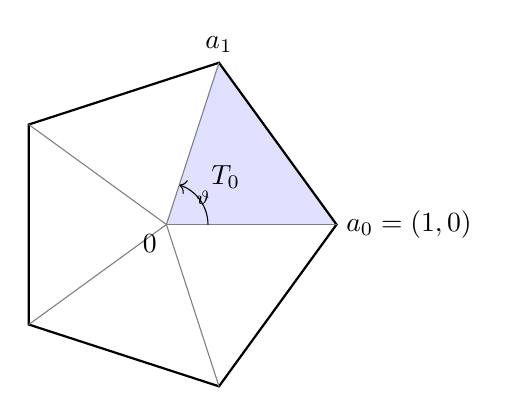
\begin{tikzpicture}[scale=1.6]
\foreach \j in {0,...,4} {\coordinate (a\j) at ({72*\j}:1.35);}
\fill[blue!12] (0,0)--(a0)--(a1)--cycle;
\draw[thick] (a0)--(a1)--(a2)--(a3)--(a4)--cycle;
\foreach \j in {0,...,4} {\draw[gray] (0,0)--(a\j);}
\node[below left] at (0,0) {$0$};
\node[right] at (a0) {$a_0=(1,0)$};
\node[above] at (a1) {$a_1$};
\node at (.47,.38) {$T_0$};
\draw[->] (.33,0) arc (0:72:.33);
\node at (.29,.21) {\scriptsize$\vartheta$};
\end{tikzpicture}
\end{center}

Let $\phi_j$ be the continuous affine hat on this coarse fan, one at
$a_j$ and zero at its other vertices, including the centre. A vertex
perturbation $q=(q_j)_{j=0}^{n-1}$, $q_j\in\R^2$, is extended into the
polygon by
\[
 \theta_q(x)=\sum_j\phi_j(x)q_j.
\]
This formula says exactly how points inside the polygon move: the map
$x\mapsto x+s\theta_q(x)$ moves the boundary vertices as prescribed and
fixes the centre. For sufficiently small $s$, it is a bi-Lipschitz map.
Its gradient is constant on each fan triangle. This last fact will be
used in every subsequent calculation.

\section{From a shape derivative to a vertex Hessian}
\label{l1:vertex}
For each vertex, $U_i=(U_i^1,U_i^2)$ collects the material derivatives of
$u$ under displacements of that vertex in the two coordinate directions.
The superscript is a component, not a derivative order. Differentiating
the pulled-back weak equation gives, for scalar $v\in H^1_0(P)$,
\begin{align}
 \int_P DU_i\nabla v={}&
 \int_P-(\nabla u\cdot\nabla v)\nabla\phi_i
 +(\nabla\phi_i\cdot\nabla v)\nabla u\notag\\
 &\quad +(\nabla\phi_i\cdot\nabla u)\nabla v+v\nabla\phi_i.
 \label{l1:material}
\end{align}
For the direction $q$, the scalar material derivative is
$u_q=\sum_iq_i\cdot U_i$. All these functions have zero Dirichlet trace
on the reference polygon: the boundary condition was pulled back before
being differentiated.

We assume Laurain's distributed formula \cite[Proposition 14]{Laurain2020}.
Its planar reduction is manuscript equation~\meq{eq:HJ}:
\begin{align}
 (D^2J)_{ij}={}&\int_P DU_iDU_j^T\notag\\
 &+\int_P\left(\tfrac12|\nabla u|^2+u\right)
 (\nabla\phi_i\otimes\nabla\phi_j-
  \nabla\phi_j\otimes\nabla\phi_i)\notag\\
 &-\int_P(\nabla\phi_i\cdot\nabla\phi_j)
              (\nabla u\otimes\nabla u).
 \label{l1:HJ}
\end{align}
This is a $2\times2$ block. For example its Gram contribution in component
$(p,q)$ is $\int_P\nabla U_i^p\cdot\nabla U_j^q$.

Here is the algebra behind the reduction. For any three planar vectors
$p,r,g$,
\begin{align*}
 &(r\cdot g)p\otimes g+(p\cdot g)g\otimes r
 -(p\cdot g)r\otimes g-(r\cdot g)g\otimes p\\
 &\hspace{25mm}=|g|^2(p\otimes r-r\otimes p).
\end{align*}
Checking the two diagonal entries gives zero on both sides; checking one
off-diagonal entry gives the other by antisymmetry. Substitute
$p=\nabla\phi_i$, $r=\nabla\phi_j$, $g=\nabla u$ in Laurain's integrand.
The remaining terms proportional to $u$ give the skew expression in
\eqref{l1:HJ}. This is a two-dimensional simplification; it should not be
used unchanged in dimension three.

There are two useful structural checks. First, individual blocks need not
be symmetric, but $(D^2J)_{ji}=((D^2J)_{ij})^T$. Second, the last two terms
are local: the hats have overlapping gradients only for identical or
neighboring vertices. The Gram term is the only generally dense part.

\subsection{The area correction must be differentiated too}
The shoelace formula gives
\[
 A=\frac12\sum_j(x_jy_{j+1}-y_jx_{j+1}),\qquad
 \nabla_{a_i}A=\frac12(y_{i+1}-y_{i-1},x_{i-1}-x_{i+1}).
\]
The only nonzero mixed second derivatives connect neighboring vertices:
$A_{x_i y_{i+1}}=1/2$ and $A_{y_i x_{i+1}}=-1/2$, together with their
symmetric counterparts. At the regular polygon,
$A=n\sin\vartheta/2$ and $\nabla_{a_i}A=\sin\vartheta\,a_i$.

By the ordinary product rule,
\begin{align}
 D^2\F={}&A^{-2}D^2J-2JA^{-3}D^2A\notag\\
 &-2A^{-3}(\nabla J\otimes\nabla A+\nabla A\otimes\nabla J)
 +6JA^{-4}\nabla A\otimes\nabla A.
 \label{l1:HFgeneral}
\end{align}
Dihedral symmetry makes $\nabla_{a_i}J$ a common multiple of $a_i$.
Euler's identity for the degree-four functional $J$ then gives
\[
 \nabla J=\frac{2J}{A}\nabla A,
 \qquad D\F(P_n)=0.
\]
Substitution into \eqref{l1:HFgeneral} yields
\begin{equation}
 D^2\F=A^{-2}D^2J-2JA^{-3}D^2A
              -2JA^{-4}\nabla A\otimes\nabla A.
 \label{l1:HF}
\end{equation}
This formula is valid at the regular polygon. On the area-tangent space,
$D^2J-(2J/A)D^2A$ has the same signs as $D^2\F$.
One must not inspect $D^2J$ alone: radial dilation increases $J$.

\section{Compute the local part on two triangles}
\label{l1:local}
The hat gradients at vertex zero are
\[
 \nabla\phi_0=(1,-\cot\vartheta)\text{ on }T_0,
 \qquad
 \nabla\phi_0=(1,\cot\vartheta)\text{ on }T_{-1},
\]
and zero elsewhere. Also,
$\nabla\phi_1=(0,1/\sin\vartheta)$ on $T_0$ and
$\nabla\phi_{-1}=(0,-1/\sin\vartheta)$ on $T_{-1}$.
These identities follow by solving the three nodal interpolation equations,
not by differentiating a trigonometric interpolant.

Only three sector integrals are needed:
\[
 X=\int_{T_0}u_x^2,\qquad Y=\int_{T_0}u_y^2,
 \qquad Z=\int_{T_0}u_xu_y.
\]
Reflection across each radial side makes $\partial_nu=0$ there.
On the polygon side $u=0$. Integration by parts within $T_0$ therefore gives
\[
 X+Y=\int_{T_0}u=\frac{2J}{n},\qquad
 \int_{T_0}(\tfrac12|\nabla u|^2+u)=\frac{3J}{n}.
\]
Reflection across the sector bisector diagonalizes the sector energy tensor
in the bisector basis. In Cartesian coordinates this means
\begin{equation}
 (Y-X)\sin\vartheta+2Z\cos\vartheta=0.
 \label{l1:sector}
\end{equation}
In particular,
$-X\sin\vartheta+Z\cos\vartheta=-J\sin\vartheta/n$.
This identity is the cancellation to remember; storing $Z$ separately is
unnecessary for the final symbol.

Write $L_j$ for the first block row of the local, non-Gram part of $D^2J$.
Substitution of the hat gradients into \eqref{l1:HJ} gives
\begin{align}
 L_0&=-\frac{2}{\sin^2\vartheta}
          \begin{pmatrix}X&0\\0&Y\end{pmatrix},\notag\\
 L_1&=\frac{\cos\vartheta}{\sin^2\vartheta}
          \begin{pmatrix}X&Z\\Z&Y\end{pmatrix}
       -\frac{3J}{n\sin\vartheta}\begin{pmatrix}0&-1\\1&0\end{pmatrix},\notag\\
 L_{-1}&=\frac{\cos\vartheta}{\sin^2\vartheta}
          \begin{pmatrix}X&-Z\\-Z&Y\end{pmatrix}
       +\frac{3J}{n\sin\vartheta}\begin{pmatrix}0&-1\\1&0\end{pmatrix}.
 \label{l1:localblocks}
\end{align}
All other $L_j$ vanish. To check the sign in $L_1$, note that
$\nabla\phi_0\cdot\nabla\phi_1=-\cos\vartheta/\sin^2\vartheta$,
whereas
$\nabla\phi_0\otimes\nabla\phi_1-
 \nabla\phi_1\otimes\nabla\phi_0$
is the negative of the displayed rotation matrix divided by
$\sin\vartheta$.

\subsection{What remains unknown in the sector integrals?}
If $\Delta_n$ denotes the difference of the energies parallel and
perpendicular to the sector bisector, rotation of that diagonal tensor gives
\[
 X=\frac Jn+\frac{\Delta_n}{2}\cos\vartheta,\quad
 Y=\frac Jn-\frac{\Delta_n}{2}\cos\vartheta,\quad
 Z=\frac{\Delta_n}{2}\sin\vartheta.
\]
Symmetry alone does not determine $\Delta_n$. The manuscript's mixed
Dirichlet--Neumann torsion problem provides an analytic characterization
of it; the fixed-mesh certificate does not need that separate computation.
For the square, $X=Y=J/4$ even though $Z$ need not vanish. The sector is
not symmetric under reflection in the Cartesian axes individually.

\section{Why radial and tangential coordinates reveal the spectrum}
\label{l1:fourier}
At vertex $j$, the radial unit vector is $a_j$ and the tangential unit
vector is $(-\sin(j\vartheta),\cos(j\vartheta))$. They are the columns
of $R_j$. With $\mathsf R=\operatorname{diag}(R_0,\ldots,R_{n-1})$, set
\[
 H=\mathsf R^TD^2\F\mathsf R.
\]
This is an orthogonal change of coordinates, so eigenvalues are unchanged.
In these coordinates rotation of the polygon merely shifts the vertex
index. Consequently $H_{ij}=C_{j-i}$, where $C_{-j}=C_j^T$.

The block-circulant reduction is due to Tee \cite{Tee2007} and is used in
this polygonal setting by Bogosel and Bucur \cite{BogoselBucur2024}.
It can be proved in one line. For a sequence
$v_j=e^{ikj\vartheta}w$, $w\in\mathbb C^2$,
\[
 (Hv)_i=\sum_j C_{j-i}e^{ikj\vartheta}w
 =e^{iki\vartheta}\left(\sum_{j=0}^{n-1}e^{ikj\vartheta}C_j\right)w.
\]
Thus the $k$th Fourier subspace carries the $2\times2$ matrix
\begin{equation}
 B_k=\sum_{j=0}^{n-1}e^{ikj\vartheta}C_j.
 \label{l1:symbol}
\end{equation}
The normalized discrete Fourier transform is unitary; the multiset of all
$2n$ Hessian eigenvalues is the union of the spectra of these $n$ blocks.

Symmetry gives $B_k^*=B_k$. Reflection in the axis through vertex zero
acts as $\operatorname{diag}(1,-1)$ on radial/tangential components and
sends $j$ to $-j$. The diagonal sequences are even and the off-diagonal
sequence is odd. Therefore
\begin{equation}
 B_k=\begin{pmatrix}\alpha_k&i\gamma_k\\-i\gamma_k&\beta_k\end{pmatrix},
 \qquad
 \mu_k^\pm=\frac{\alpha_k+\beta_k
 \pm\sqrt{(\alpha_k-\beta_k)^2+4\gamma_k^2}}2.
 \label{l1:eigenvalues}
\end{equation}
The parameters $\alpha_k,\beta_k,\gamma_k$ are real. These are manuscript
equations (\meq{eq:symbol-entries})--(\meq{eq:mode-eigs}). The sign of the imaginary
entry depends on the Fourier convention; the convention in
\eqref{l1:symbol} is fixed throughout these notes.

\subsection{The explicit cancellation with area}
The radial/tangential area symbol is
\[
 \sin\vartheta\cos(k\vartheta)I
 -i\cos\vartheta\sin(k\vartheta)
                  \begin{pmatrix}0&-1\\1&0\end{pmatrix}.
\]
In the first row, the local blocks become $L_jR_j$, since $R_0=I$.
Multiply the three matrices in \eqref{l1:localblocks} by $R_j$, use
\eqref{l1:sector}, and subtract the area contribution in \eqref{l1:HF}.
The result is
\begin{align}
 &A^{-2}\sum_{j=-1}^{1}e^{ikj\vartheta}L_jR_j
 -2JA^{-3}\left[\sin\vartheta\cos(k\vartheta)I
 -i\cos\vartheta\sin(k\vartheta)
       \begin{pmatrix}0&-1\\1&0\end{pmatrix}\right]\notag\\
 &\hspace{15mm}=-\frac{2(1-\cos(k\vartheta))}{A^2\sin^2\vartheta}
                    \begin{pmatrix}X&0\\0&Y\end{pmatrix}.
 \label{l1:cancellation}
\end{align}
The explicit off-diagonal term disappears completely. The rank-one term
$\nabla A\otimes\nabla A$ in \eqref{l1:HF} acts only on the constant
radial sequence, hence only on mode zero.

For clarity, introduce the scalar rotated components already used in the
manuscript:
\[
 U_{j,r}=\cos(j\vartheta)U_j^1+\sin(j\vartheta)U_j^2,\quad
 U_{j,t}=-\sin(j\vartheta)U_j^1+\cos(j\vartheta)U_j^2,
 \qquad a(v,w)=\int_P\nabla v\cdot\nabla w.
\]
The three genuinely nonlocal quantities are
\begin{align*}
 G^{rr}_k&=\sum_j\cos(kj\vartheta)a(U_0^1,U_{j,r}),\\
 G^{tt}_k&=\sum_j\cos(kj\vartheta)a(U_0^2,U_{j,t}),\\
 G^{rt}_k&=\sum_j\sin(kj\vartheta)a(U_0^1,U_{j,t}).
\end{align*}
For every nonzero mode, \eqref{l1:cancellation} now yields
\begin{equation}
 \boxed{\begin{aligned}
 \alpha_k&=A^{-2}\left[G^{rr}_k-
          \frac{2(1-\cos(k\vartheta))X}{\sin^2\vartheta}\right],\\
 \beta_k&=A^{-2}\left[G^{tt}_k-
          \frac{2(1-\cos(k\vartheta))Y}{\sin^2\vartheta}\right],\\
 \gamma_k&=A^{-2}G^{rt}_k.
 \end{aligned}}
 \label{l1:finalentries}
\end{equation}
These are the requested Hessian eigenvalue formulas together with
\eqref{l1:eigenvalues}. Their trace contains the explicit penalty
$-4(1-\cos(k\vartheta))J/(nA^2\sin^2\vartheta)$.
Sector anisotropy cancels from that explicit penalty; it does not cancel
from the state-dependent Gram terms.

\section{Exact zero modes and the local maximum criterion}
\label{l1:zeros}
At a critical point of a similarity-invariant function, differentiating
invariance puts the four infinitesimal similarity directions in the Hessian
kernel. The mode bookkeeping matters:
\begin{center}
\begin{tabular}{lll}\toprule
motion & radial/tangential coordinates & Fourier location\\\midrule
scaling & $(1,0)$ at every vertex & $k=0$\\
rotation & $(0,1)$ at every vertex & $k=0$\\
$x$ translation & $(\cos(j\vartheta),-\sin(j\vartheta))$ & $k=1,n-1$\\
$y$ translation & $(\sin(j\vartheta),\cos(j\vartheta))$ & $k=1,n-1$\\\bottomrule
\end{tabular}
\end{center}
Thus $B_0=0$. At $k=1$ the complex translation vector is $(1,i)$, so
$\alpha_1=\beta_1=\gamma_1$. The other eigenvalue is the trace
$\alpha_1+\beta_1$. The conjugate mode $n-1$ gives the other real
translation and the same nonzero eigenvalue.

Also $B_{n-k}=\overline{B_k}$. If $n$ is even, the Nyquist mode $k=n/2$
has zero sine sequence and $\gamma_{n/2}=0$. These are exact identities,
not quantities to be recognized by a small numerical threshold.
For a generic block, strict negativity is equivalent to
\[
 \alpha_k+\beta_k<0,\qquad \alpha_k\beta_k-\gamma_k^2>0.
\]
This determinant test excludes translation blocks, whose determinant is
exactly zero; there the trace alone is tested.

\begin{theorem}[What the numerical calculation must establish]
If every branch outside the four similarity directions is strictly
negative, the regular polygon is a strict local maximizer of $J/A^2$
modulo similarities. Equivalently, it is a strict local maximizer of $J$
at fixed area, modulo translations and rotations.
\end{theorem}
\begin{proof}
The fan pullback has smoothly parameter-dependent, uniformly elliptic
coefficients in a sufficiently small vertex neighborhood. Its inverse
solution operator is smooth, so the objective is twice differentiable.
Choose a local slice complementary to the four-dimensional similarity
orbit. The Hessian is negative definite on the slice; Taylor's theorem
gives strict decrease for small nonzero slice displacements. Every nearby
orbit meets the slice. Fixing area removes the dilation freedom.
This proves a local statement about nearby labelled polygons, not global
optimality among all polygons.
\end{proof}

\section{The quantities actually passed to the next lecture}
\label{l1:pairings}
One need not assemble the entire Hessian to evaluate its symbol. For
$1\leq k<n/2$, the following are normalized vertex displacements:
\begin{align*}
 r^c_{k,j}&=\sqrt{2/n}\cos(kj\vartheta)
                     (\cos(j\vartheta),\sin(j\vartheta)),
                     &&\text{radial, cosine},\\
 t^c_{k,j}&=\sqrt{2/n}\cos(kj\vartheta)
                     (-\sin(j\vartheta),\cos(j\vartheta)),
                     &&\text{tangential, cosine},\\
 t^s_{k,j}&=\sqrt{2/n}\sin(kj\vartheta)
                     (-\sin(j\vartheta),\cos(j\vartheta)),
                     &&\text{tangential, sine}.
\end{align*}
Their pairings give respectively
\[
 D^2\F[r_k^c,r_k^c]=\alpha_k,\quad
 D^2\F[t_k^c,t_k^c]=\beta_k,\quad
 D^2\F[r_k^c,t_k^c]=0,\quad
 D^2\F[r_k^c,t_k^s]=\gamma_k.
\]
For the Nyquist cosine directions use $(-1)^j/\sqrt n$ instead of
$\sqrt{2/n}\cos(kj\vartheta)$. The certificate encloses these real
pairings directly; it need not compute separate intervals for $X,Y,Z$
or the Gram sums.

Finally, covariance gives
\[
 U_j(x)=R_jU_0(R_j^Tx),\qquad
 U_{j,r}(x)=U_0^1(R_j^Tx),\qquad
 U_{j,t}(x)=U_0^2(R_j^Tx).
\]
The distinction between vector rotation and scalar pullback explains the
optimized code: torsion and two first-vertex PDEs supply every first
material derivative. Later second-lifting solves serve error estimation.

\subsection*{Exercises and answers for discussion}
\begin{exercise}
Derive $\nabla J=(2J/A)\nabla A$ without a boundary integral formula.
\end{exercise}
\noindent\emph{Answer.} Reflection makes each gradient radial; rotation
makes their coefficients equal. If $\nabla_{a_j}J=c a_j$, Euler's identity
gives $nc=4J$. Compare with $\nabla_{a_j}A=\sin\vartheta a_j$.

\begin{exercise}
For $n=5$, explain why the target is six negative eigenvalues, even though
there are only two representative nonzero modes.
\end{exercise}
\noindent\emph{Answer.} Modes $1,4$ contribute one physical eigenvalue each;
modes $2,3$ contribute two each. Mode zero and the two translations supply
four zeros. The total is $2+4=6$ negatives out of ten dimensions.

\begin{exercise}
Can a negative computed trace alone certify a generic $2\times2$ block?
\end{exercise}
\noindent\emph{Answer.} No. A block with eigenvalues $-2$ and $1$ has
negative trace. A determinant bound or two strictly negative eigenvalue
enclosures is also required.

\clearpage
\part{Finite element errors, fluxes, and transmission regularity}
\section{Three errors that must not be confused}
\label{l2:errors}
\noindent\textbf{Aim.} Turn a finite element Hessian entry into an enclosure
of the continuous entry. Then investigate the transmission regularity
behind its observed quadratic convergence. A 90-minute lecture can cover
the error identities and first-derivative regularity; the second-derivative
argument below is suitable for a further reading session.

The geometry is the same regular polygon and coarse fan as in the first
lecture. Write $a(v,w)=\int_P\nabla v\cdot\nabla w$ and
$\energy v=\|\nabla v\|_{L^2(P)}$. A displacement $q$ has the fan extension
$\theta_q=\sum_jq_j\phi_j$. These are vertex displacements, not functions
that can be chosen independently on adjacent triangles.
Recall that $-\Delta u=1$, $u\in H^1_0(P)$, $\ell(v)=\int_Pv$,
$J=\frac12\int_Pu$, and $\F=J/A^2$ with $A=|P|$.

There are three distinct objects:
\begin{center}
\begin{tabular}{lll}\toprule
object & meaning & source of the difference\\\midrule
$u$ & continuous weak solution & ---\\
$u_h$ & exact Galerkin solution in $V_h$ & spatial discretization\\
$\widetilde u$ & computed coefficient vector in $V_h$ & linear-system solve\\\bottomrule
\end{tabular}
\end{center}
Interval rounding is a third error, incurred while evaluating quantities
in the proof. It is handled by enclosing each arithmetic operation.
A small solver residual alone controls neither $u-u_h$ nor the Hessian
error. Conversely, an a priori interpolation theorem does not control the
rounding error in a computed residual.

Each coarse triangle is split uniformly into $m^2$ fine triangles. The
mesh has $nm^2$ triangles and $1+nm(m+1)/2$ vertices. Its boundary has
$nm$ vertices. For fixed $n$, $h=m^{-1}$ is proportional to the maximum
fine-element diameter. All rays are unions of element edges, and the
coefficients obtained by differentiating the pullback are constant on each
fine triangle. A mesh crossing a ray cannot use the same broken
interpolation argument without additional analysis.
The space $V_h$ consists of continuous functions that are affine on each
fine triangle and zero on the polygon boundary. The exact Galerkin state
is characterized by $a(u_h,v_h)=\ell(v_h)$ for every $v_h\in V_h$.
It is a mathematical solution of a finite linear system, independently
of how accurately a numerical solver finds its coefficients.

\section{A residual is an error measured in the dual norm}
\label{l2:residual}
For $u$ satisfying $a(u,v)=\ell(v)$ and any conforming candidate $w$,
\[
 a(u-w,v)=\ell(v)-a(w,v).
\]
Taking the supremum over $\energy v=1$ gives an equality:
\[
 \energy{u-w}=\|\ell-a(w,\cdot)\|_{(H^1_0,a)^*}.
\]
The equality does not compute the dual norm. It identifies what a guaranteed
majorant must bound.

For torsion, let $y\in H(\operatorname{div};P)$ satisfy
$\operatorname{div}y=-1$. Integration by parts, with the zero trace of $v$,
gives
\[
 \ell(v)-a(w,v)=\int_P(y-\nabla w)\cdot\nabla v,
 \qquad \energy{u-w}\leq\|y-\nabla w\|_{L^2(P)}.
\]
This is a guaranteed estimate: it is valid for every admissible $y$, not
only the minimizer of a flux-fitting problem. It is a functional majorant
in the sense discussed by Repin and by the guaranteed finite element
literature \cite{Repin2008,LiuOishi2013,LiLiu2018}.

A convenient exact construction is
\begin{equation}
 y=-x/2+\curl\psi_h,
 \qquad \curl\psi_h=(\partial_y\psi_h,-\partial_x\psi_h),
 \label{l2:flux0}
\end{equation}
where $\psi_h$ is continuous and piecewise affine. In distributions,
$\operatorname{div}\curl\psi_h=0$. Across an element edge the normal
component of the curl is a tangential derivative of the common trace of
$\psi_h$, so it agrees from both sides. Thus this is a global
$H(\operatorname{div})$ field with precisely the required divergence.

The numerical code chooses $\psi_h$ by minimizing a quadratic mismatch.
Its computed nodal values are simply admissible flux data. An inaccurate
fit widens the bound; it does not destroy equilibration. The first part
$-x/2$ is essential: a curl alone would have the wrong divergence.

\begin{exercise}
What happens if the flux is not exactly equilibrated?
\end{exercise}
\noindent\emph{Answer.} The still-valid estimate is
$\energy{u-w}\leq\|y-\nabla w\|+C_F\|1+\operatorname{div}y\|$,
where $\|v\|\leq C_F\energy v$. Exact equilibration removes the second term.

\section{Differentiate the weak problem, not the approximate output}
\label{l2:pullback}
For two vertex directions, use
$x\mapsto x+s\theta_q(x)+t\theta_r(x)$. The pulled-back coefficient matrix
and volume density are
\[
 \mathbb A(s,t)=\det(I+sD\theta_q+tD\theta_r)
 (I+sD\theta_q+tD\theta_r)^{-1}
 (I+sD\theta_q+tD\theta_r)^{-T},
\]
\[
 a_{s,t}(v,w)=\int_P\nabla v^T\mathbb A(s,t)\nabla w,
 \qquad
 \ell_{s,t}(v)=\int_P\det(I+sD\theta_q+tD\theta_r)v.
\]
Subscripts $q,r,qr$ on forms mean derivatives at $s=t=0$.
In particular,
\begin{align*}
 \mathbb A_q&=(\operatorname{div}\theta_q)I-D\theta_q-D\theta_q^T,\\
 \ell_q(v)&=\int_P(\operatorname{div}\theta_q)v,\\
 \ell_{qr}(v)&=\int_P\big[(\operatorname{div}\theta_q)
 (\operatorname{div}\theta_r)-\tr(D\theta_qD\theta_r)\big]v.
\end{align*}
Differentiating $a_{s,t}(u_{s,t},v)=\ell_{s,t}(v)$ gives
\begin{align}
 a(u_q,v)&=\ell_q(v)-a_q(u,v),\notag\\
 a(u_{qr},v)&=\ell_{qr}(v)-a_q(u_r,v)-a_r(u_q,v)-a_{qr}(u,v).
 \label{l2:exactderivatives}
\end{align}
All derivatives here are material derivatives on the fixed reference fan.
They exist in $H^1_0$ by differentiability of the uniformly coercive
solution operator; that fact alone does not give broken $H^2$ regularity.

Replace the test space by $V_h$ and the state by $u_h$. The exact discrete
first derivatives solve the resulting equations, and $z_h=u_{h,qr}$
solves the fourth discrete equation. Define the continuous lifting by
\begin{equation}
 a(Z_{qr}^h,v)=\ell_{qr}(v)-a_q(u_{h,r},v)
                    -a_r(u_{h,q},v)-a_{qr}(u_h,v).
 \label{l2:lifting}
\end{equation}
Its Galerkin solution is $z_h$. The superscript $h$ on $Z_{qr}^h$ refers
to its data; $Z_{qr}^h$ itself is not a finite element function.

The following form bounds are finite maxima of matrix operator norms:
\[
 |a_q(v,w)|\leq C_q\energy v\energy w,\quad
 |a_r(v,w)|\leq C_r\energy v\energy w,\quad
 |a_{qr}(v,w)|\leq C_{qr}\energy v\energy w.
\]
They transfer errors between the successive equations. No smallness of
$C_q,C_r,C_{qr}$ is assumed.

\section{Why the second variation admits products of errors}
\label{l2:identity}
Set $e=u-u_h$, $e_q=u_q-u_{h,q}$, and $e_r=u_r-u_{h,r}$.
Galerkin orthogonality gives the exact identity
\begin{equation}
 J-J_h=\tfrac12a(e,e).
 \label{l2:energyidentity}
\end{equation}
It holds on nearby polygons after pullback. Differentiating twice means
differentiating the form as well as both arguments:
\[
 (J-J_h)_{qr}=\tfrac12a_{qr}(e,e)+a_q(e_r,e)+a_r(e_q,e)
                      +a(e_q,e_r)+a(e_{qr},e).
\]
Since $u_{h,qr}\in V_h$, orthogonality gives
$a(e_{qr},e)=a(u_{qr},e)$. Insert the second equation in
\eqref{l2:exactderivatives}, tested with $e$, and combine the terms.
The result is
\begin{equation}
 (J-J_h)_{qr}=a(e_q,e_r)-\tfrac12a_{qr}(e,e)
                         +a(Z_{qr}^h-z_h,e).
 \label{l2:productidentity}
\end{equation}
The exact second derivative has disappeared. If
\[
 \energy e\leq\delta_0,\quad \energy{e_q}\leq\delta_q,
 \quad\energy{e_r}\leq\delta_r,\quad
 \energy{Z_{qr}^h-z_h}\leq\eta_{qr},
\]
then
\begin{equation}
 |(J-J_h)_{qr}|\leq
 \delta_q\delta_r+\tfrac12C_{qr}\delta_0^2+\delta_0\eta_{qr}.
 \label{l2:productbound}
\end{equation}
This is manuscript equation~\meq{eq:second-residual-bound}.
It is valid on each fixed mesh without an asymptotic regularity assumption.

\subsection{Could we use only material derivatives?}
Yes. The weak equation already gives
$a(u_q,u_r)=\ell_q(u_r)-a_q(u,u_r)$. It uses no second derivative.
But replacing $u$ by $u_h$ changes the load, so it does not automatically
remove the terms linear in the state error. Direct propagation of
$O(h)$ energy bounds through the Hessian generally leaves an $O(h)$ bound.
The Bogosel--Bucur analysis already exploits a quadratic interpolation
product for material derivatives; the leading first-order contribution
comes from other data errors, not a failure of Galerkin orthogonality
\cite[Section 3.1]{BogoselBucurValidated2024}.

In \eqref{l2:productbound}, all four errors of order $h$ instead produce
an order-$h^2$ bound. This improvement is due to the cancellation and
lifting. Equilibrated fluxes are a way to enclose the energy errors;
they are not, by themselves, a theorem of quadratic convergence.

\section{The computed linear systems also need error bounds}
\label{l2:algebraic}
Let $Kx_*=f$ be the exact interior-node system, with $K$ symmetric positive
definite. A computed vector $x$ has residual $f-Kx$. If
$\lambda_{\min}(K)\geq\underline\alpha>0$, then
\[
 \|x-x_*\|_K^2=(f-Kx)^TK^{-1}(f-Kx)
 \leq \frac{\|f-Kx\|_2^2}{\underline\alpha}.
\]
The Euclidean norm of the residual is not the energy norm of the error;
the factor $1/\sqrt{\underline\alpha}$ supplies that conversion.

For the circumradius-one polygon, domain monotonicity and the square give
$\lambda_1(P)\geq\pi^2/2$. On one triangle,
\[
 M_T=\frac{|T|}{12}
 \begin{pmatrix}2&1&1\\1&2&1\\1&1&2\end{pmatrix}
 \succeq\frac{|T|}{12}I.
\]
After assembly and restriction to interior nodes,
\begin{equation}
 \underline\alpha=
 \frac{\pi^2}{24}\min_{i\text{ interior}}\sum_{T\ni i}|T|
 \quad\hbox{is a valid lower bound for }\lambda_{\min}(K).
 \label{l2:coercivity}
\end{equation}
This is explicit and possibly conservative. It contains no numerically
estimated inverse and no uncertified eigenvalue computation.

Define the four residual functionals of the computed candidates:
\begin{align*}
 \rho_0(v)&=\ell(v)-a(\widetilde u,v),\\
 \rho_q(v)&=\ell_q(v)-a_q(\widetilde u,v)-a(\widetilde u_q,v),\\
 \rho_r(v)&=\ell_r(v)-a_r(\widetilde u,v)-a(\widetilde u_r,v),\\
 \rho_z(v)&=\ell_{qr}(v)-a_q(\widetilde u_r,v)
 -a_r(\widetilde u_q,v)-a_{qr}(\widetilde u,v)-a(\widetilde z,v).
\end{align*}
Their vectors are obtained by evaluating them on each interior basis
function $\varphi_i$: $(r_\rho)_i=\rho(\varphi_i)$. For example,
$r_{\rho_0}=f-K\widetilde x$.

Because later loads contain earlier unknowns, the transfer is
\begin{align*}
 \epsilon_0&=\|r_{\rho_0}\|_2/\sqrt{\underline\alpha},\\
 \epsilon_q&=\|r_{\rho_q}\|_2/\sqrt{\underline\alpha}+C_q\epsilon_0,\\
 \epsilon_r&=\|r_{\rho_r}\|_2/\sqrt{\underline\alpha}+C_r\epsilon_0.
\end{align*}
These bound the differences between exact discrete solutions and their
candidates. Boundary coefficients are set to exactly zero before any
residual is assembled. A large penalty imposed by a floating-point
solver is not a substitute for this Dirichlet restriction.

\subsection{Correct the centre before increasing the radius}
The energy centre
$\widetilde J_{\rm corr}=\ell(\widetilde u)-a(\widetilde u,\widetilde u)/2$
satisfies $J_h-\widetilde J_{\rm corr}=\energy{u_h-\widetilde u}^2/2$.
For the mixed derivative use
\begin{align*}
 \widetilde C_{\rm corr}={}&\ell_{qr}(\widetilde u)
 +\ell_q(\widetilde u_r)-\tfrac12a_{qr}(\widetilde u,\widetilde u)
 -a_q(\widetilde u,\widetilde u_r)\\
 &+\rho_r(\widetilde u_q)+\rho_0(\widetilde z).
\end{align*}
Expanding about the exact discrete fields and substituting the residual
identities gives
\begin{align*}
 J_{h,qr}-\widetilde C_{\rm corr}
 ={}&\rho_z(u_h-\widetilde u)
 -\tfrac12a_{qr}(u_h-\widetilde u,u_h-\widetilde u)\\
 &+a(u_{h,q}-\widetilde u_q,u_{h,r}-\widetilde u_r).
\end{align*}
Every first-order material-solve term has cancelled. Consequently
\[
 |J_{h,qr}-\widetilde C_{\rm corr}|\leq E_{\rm alg}
 :=\frac{\|r_{\rho_z}\|_2}{\sqrt{\underline\alpha}}\epsilon_0
   +\tfrac12C_{qr}\epsilon_0^2+\epsilon_q\epsilon_r.
\]
The lifting solve error need not be given another separate name: its
residual appears directly in this expression.

\section{Four fluxes and the final continuous enclosure}
\label{l2:assembly}
Choose four continuous affine potentials. The state flux is
\eqref{l2:flux0}; the first-derivative flux is
$-\theta_q+\curl\psi_{q,h}$, with divergence $-\operatorname{div}\theta_q$.
For the second lifting use
\[
 -(\operatorname{div}\theta_q)\theta_r+D\theta_q\theta_r
                                  +\curl\psi_{z,h}.
\]
Indeed,
\[
 \operatorname{div}\big((\operatorname{div}\theta_q)\theta_r
                 -D\theta_q\theta_r\big)
 =(\operatorname{div}\theta_q)(\operatorname{div}\theta_r)
                       -\tr(D\theta_qD\theta_r).
\]
Its normal trace is continuous across fan edges: the gradient jump of a
continuous affine field is a vector tensor the edge normal, and the two
normal jump contributions cancel. This is a distributional identity,
not only a trianglewise identity.

The four mismatch norms are
\begin{align*}
 \Phi_0&=\|-x/2+\curl\psi_{0,h}-\nabla\widetilde u\|,\\
 \Phi_q&=\|-\theta_q+\curl\psi_{q,h}-\nabla\widetilde u_q
                                     -\mathbb A_q\nabla\widetilde u\|,\\
 \Phi_r&=\|-\theta_r+\curl\psi_{r,h}-\nabla\widetilde u_r
                                     -\mathbb A_r\nabla\widetilde u\|,\\
 \Phi_z&=\|-(\operatorname{div}\theta_q)\theta_r+D\theta_q\theta_r
                 +\curl\psi_{z,h}-\nabla\widetilde z\\
 &\hspace{23mm}-\mathbb A_q\nabla\widetilde u_r
                 -\mathbb A_r\nabla\widetilde u_q
                 -\mathbb A_{qr}\nabla\widetilde u\|.
\end{align*}
All unmarked norms in these formulas are $L^2(P)$ norms of vector fields.
Residual bounds, load-error transfer, and best approximation give
\begin{align*}
 \widehat\delta_0&=\Phi_0,\\
 \widehat\delta_q&=\Phi_q+C_q\Phi_0+\epsilon_q,
 &\widehat\delta_r&=\Phi_r+C_r\Phi_0+\epsilon_r,\\
 \widehat\eta_{qr}&=\Phi_z+C_q\epsilon_r+C_r\epsilon_q+C_{qr}\epsilon_0.
\end{align*}
For example, $\Phi_0$ bounds the error to $\widetilde u$; best
approximation then also bounds the error to $u_h$. In the lifting bound,
$\widetilde z\in V_h$ can replace $z_h$ before best approximation is used.
This explains why an extra lifting algebraic error is not added there.

For a nonzero Fourier pairing, $A_q=A_r=0$. Define
\[
 B_J=\widehat\delta_q\widehat\delta_r+\tfrac12C_{qr}\widehat\delta_0^2
                           +\widehat\delta_0\widehat\eta_{qr}.
\]
The entry centre and radius are
\begin{align}
 \widetilde F_{qr}&=\frac{\widetilde C_{\rm corr}}{A^2}
                     -\frac{2\widetilde J_{\rm corr}A_{qr}}{A^3},\notag\\
 R_F&=\frac{B_J+E_{\rm alg}}{A^2}
       +\frac{|A_{qr}|}{A^3}(\widehat\delta_0^2+\epsilon_0^2),\notag\\
 |D^2\F[q,r]-\widetilde F_{qr}|&\leq R_F.
 \label{l2:finalradius}
\end{align}
Every term has a job: $B_J$ is the continuous discretization error,
$E_{\rm alg}$ is the error in the discrete centre, and the last term
accounts for the area-normalization coefficient multiplying $J$.
If the evaluated centre is an interval, its arithmetic radius is retained.

\section{Regularity attempt: integrate the vertex-zero load by parts}
\label{l2:rayproof}
This section develops the proposed Bogosel--Bucur route. We will prove
broken regularity of first and second material derivatives \emph{at the
regular polygon}, using the standard polygonal mixed-boundary regularity
theorem stated below. A separate final paragraph explains why this does
not yet prove the manuscript's stronger uniform-neighborhood formulation.

For $c=1,2$, put the weak equation for $U_0^c$ in the form
\begin{align}
 a(U_0^c,v)&=\int_P G_{0,c}(u)\cdot\nabla v
                              +\int_P(\partial_c\phi_0)v,\notag\\
 G_{0,c}(u)&=-(\partial_c\phi_0)\nabla u
            +(\partial_cu)\nabla\phi_0
            +(\nabla\phi_0\cdot\nabla u)e_c.
 \label{l2:G}
\end{align}
On a sector the hat gradient is constant. Since $\Delta u=-1$,
\[
 \operatorname{div}G_{0,c}(u)
 =\partial_c\phi_0+2\nabla\phi_0\cdot\nabla\partial_cu.
\]
The volume load after integration by parts is therefore
\begin{equation}
 -2\nabla\phi_0\cdot\nabla\partial_cu\in L^2(P).
 \label{l2:regularload}
\end{equation}
It is supported on $T_{-1}\cup T_0$. The term
$\partial_c\phi_0$ has cancelled; keeping it would give an incorrect
strong formulation.

Let $S_j=\{r a_j:0<r<1\}$ and let
$\nu_j=(-\sin(j\vartheta),\cos(j\vartheta))$ point from $T_{j-1}$ into
$T_j$. The trace convention is $[w]_j=w|_{T_j}-w|_{T_{j-1}}$.
The contribution of the two boundary integrals is
$-[G_{0,c}(u)]_j\cdot\nu_j$.
Continuity of $\phi_0$ implies $[\nabla\phi_0]_j$ is normal to $S_j$.
Because $u\in H^2(P)$, its gradient has a common trace there. Substituting
into \eqref{l2:G} gives the especially simple ray density
\begin{equation}
 -[G_{0,c}(u)]_j\cdot\nu_j
     =-([\nabla\phi_0]_j\cdot\nu_j)\,\partial_cu|_{S_j}.
 \label{l2:raydensity}
\end{equation}
Only $S_{-1},S_0,S_1$ occur. Their coefficients are
\[
 [\nabla\phi_0]_0\cdot\nu_0=-2\cot\vartheta,
 \qquad
 [\nabla\phi_0]_{\pm1}\cdot\nu_{\pm1}=\frac1{\sin\vartheta}.
\]
Thus the complete distributional equation is
\begin{equation}
 -\Delta U_0^c=-2\nabla\phi_0\cdot\nabla\partial_cu
 +2\cot\vartheta\,(\partial_cu)|_{S_0}\delta_{S_0}
 -\frac{(\partial_cu)|_{S_1}\delta_{S_1}
        +(\partial_cu)|_{S_{-1}}\delta_{S_{-1}}}{\sin\vartheta}.
 \label{l2:decomposition}
\end{equation}
Here $g\delta_S$ means the functional $v\mapsto\int_Sgv\,ds$.
No point masses occur: we integrated bounded piecewise coefficients times
$H^1$ gradient fields once, and the singular terms are edge measures.

\subsection{Why the ray densities have the right endpoint behavior}
For fixed $n$, convex-polygon Dirichlet regularity gives
\[
 u\in H^{2+\sigma}(P),\qquad
 0<\sigma<\min\left\{\frac12,\frac{\pi}{\pi-2\pi/n}-1\right\},
\]
after decreasing $\sigma$ if necessary. Possible resonant logarithmic
corner terms are harmless below this strict exponent threshold.
In particular $\nabla u$ is continuous up to each corner. Its tangential
derivatives on the two adjacent Dirichlet edges are zero; the tangents
are independent, so $\nabla u(a_j)=0$. At the centre, rotational symmetry
implies $\nabla u(0)=0$.

On $S_j$, reflection gives zero normal derivative, hence
\[
 \nabla u(r a_j)=a_j\,\partial_ru(r,0).
\]
Thus the densities in \eqref{l2:decomposition} are precisely rotated
multiples of the same radial derivative. The trace theorem gives
$H^{1/2+\sigma}$ regularity on each ray, and the values at $r=0,1$ vanish.
Their extensions by zero across the centre belong to the same fractional
space for sufficiently small $\sigma>0$. Endpoint values here are justified
by the extra positive regularity; bare $H^{1/2}$ membership would not by
itself justify a pointwise endpoint argument.

\subsection{The mixed-boundary ingredient, with its hypotheses visible}
\begin{lemma}[A ray load with vanishing endpoints]
\label{l2:raylemma}
Fix a regular polygon. Let $g\in H^{1/2+\sigma}(0,1)$ with $g(0)=g(1)=0$
and $\sigma>0$ sufficiently small. The solution $W\in H^1_0(P)$ of
$a(W,v)=\int_{S_0}gv$ belongs to $H^{2+\sigma'}$ on each side of the ray
and on every fan sector, for some $\sigma'>0$ that may be smaller than
$\sigma$. The same assertion holds for any rotated ray.
\end{lemma}
\begin{proof}
The line load is continuous on $H^1_0(P)$ by the trace theorem, so
Lax--Milgram gives $W$. Its data and domain are invariant under reflection
across the line through $S_0$, hence $W$ is even. Restrict to the upper
half-polygon. The boundary conditions are Dirichlet zero on the polygon
boundary and outward Neumann data $g/2$ on the positive part of the cut,
zero on its negative part. The factor $1/2$ follows by doubling the weak
integral over the half-polygon.

Apply the polygonal Dirichlet--Neumann shift theorem of Grisvard
\cite[Theorem 4.4.3.7 and Corollary 4.4.3.8]{Grisvard1985}.
Its use here is the same as the
ray decomposition in \cite[Section 3]{BogoselBucurValidated2024}; the local
reviewed PDF has Lemma 3.1 and Remark 3.2. The hypotheses can be checked
geometrically. At a vertex on the cut the mixed angle is
$(\pi-\vartheta)/2<\pi/2$, whose first mixed corner exponent is
$\pi/(\pi-\vartheta)>1$. Other Dirichlet angles are less than $\pi$.
When $n$ is odd, the negative cut meets the opposite edge at a right angle;
the Neumann data are identically zero near that point, and even reflection
reduces the local problem to a straight Dirichlet boundary. There is no
nonpolynomial corner singularity of exponent at most one there.
The Neumann datum extends through the centre in $H^{1/2+\sigma}$,
and its zero value at the positive endpoint supplies the compatibility
with the zero Dirichlet data. These facts give a positive shift above
$H^2$, after shrinking the exponent. Reflection back gives the assertion.
Away from the loaded positive ray, the equation is locally harmonic across
the artificial negative cut, so no extra interface is introduced.
\end{proof}

\begin{proposition}[First material derivatives at the regular polygon]
\label{l2:firstregular}
For every fixed $n\geq3$, the first vertex material derivatives are in
$H^{2+\sigma}$ on each coarse fan triangle for some $\sigma>0$ depending
on $n$. Their gradients have a common value at the centre and vanish at
the polygon vertices.
\end{proposition}
\begin{proof}
Split \eqref{l2:decomposition} into its volume solution and three ray
solutions. The volume load is piecewise $H^\sigma$, hence globally
$H^\sigma$ after choosing $\sigma<1/2$; multiplication by a sector
indicator preserves $H^\sigma$ in this range. The convex Dirichlet
polygonal shift theorem gives $H^{2+\sigma}$ for its solution, with a
possibly smaller positive exponent. Lemma~\ref{l2:raylemma} handles the
three ray solutions. Rotation and linear combination handle all vertices
and all directions $q$.

The one-sided gradients are continuous to sector endpoints by Sobolev
embedding. Across a ray, the tangential gradient agrees, because the
function has one common trace. The normal-gradient jump equals the line
density, up to the chosen orientation. That density vanishes at both
endpoints, so the gradients agree at the centre and at each outer endpoint.
At a polygon vertex the common gradient is orthogonal to both adjacent
boundary tangents, hence is zero. At the centre the common gradient need
not be zero; symmetry of the state does not imply the same symmetry for
a single-vertex material derivative.
\end{proof}

\section{The second derivatives: a necessary centre cancellation}
\label{l2:secondregular}
The first-derivative proof is not automatically a proof for $u_{qr}$.
Nevertheless it supplies the extra regularity needed to continue. On each
sector write its weak equation as
\[
 a(u_{qr},v)=\int_P d_{qr}v+\int_P G_{qr}\cdot\nabla v,
\]
where, for this regularity calculation only,
\begin{align*}
 d_{qr}&=(\operatorname{div}\theta_q)(\operatorname{div}\theta_r)
                               -\tr(D\theta_qD\theta_r),\\
 G_{qr}&=-\mathbb A_q\nabla u_r-\mathbb A_r\nabla u_q
                                  -\mathbb A_{qr}\nabla u.
\end{align*}
These two names display the volume and flux parts of one distribution;
they do not introduce any new PDE solves. Sectorwise integration by parts
produces $d_{qr}-\operatorname{div}G_{qr}\in L^2$ and ray densities
$-[G_{qr}]_j\cdot\nu_j\in H^{1/2+\sigma}(S_j)$.
All outer endpoint values vanish by Proposition~\ref{l2:firstregular}.
The centre values may not vanish because $\nabla u_q(0)$ and
$\nabla u_r(0)$ may be nonzero.

This matters. A constant load on a ray ending at an interior point can
produce an $r\log r$ corner term; its second derivatives are not square
integrable near that endpoint. Splitting a compatible collection of rays
into unrelated single-ray problems can therefore destroy the regularity
one is trying to prove.

\subsection{An explicit local lifting removes the centre values}
Choose a smooth cutoff $\chi$ supported in an interior disk around the
centre, equal to one in a smaller disk. Subtract from $u_{qr}$ the known
piecewise smooth function
\begin{equation}
 \chi(x)\bigl(\theta_q(x)\cdot\nabla u_r(0)
                  +\theta_r(x)\cdot\nabla u_q(0)\bigr).
 \label{l2:centerlifting}
\end{equation}
It belongs to $H^1_0(P)$ and is $H^2$ on each fan sector. Its purpose is
local regularity analysis; it is not the numerical second lifting $Z_{qr}^h$.
The centre gradients are well defined by the first-derivative proposition.

For any constant vector $b$, the following identity holds in distributions:
\begin{equation}
 \operatorname{div}(-\mathbb A_q b)
     =\Delta(\theta_q\cdot b).
 \label{l2:centeridentity}
\end{equation}
Indeed,
$-\mathbb A_qb=D\theta_qb+D\theta_q^Tb-(\operatorname{div}\theta_q)b$.
The divergences of the first and last terms cancel by commutation of
weak derivatives; the middle term is $\nabla(\theta_q\cdot b)$.
Near the centre, where $\chi=1$, identity~\eqref{l2:centeridentity} shows
that \eqref{l2:centerlifting} has exactly the ray-jump contributions of
$-\mathbb A_q\nabla u_r(0)-\mathbb A_r\nabla u_q(0)$.
Also $\nabla u(0)=0$, so the $\mathbb A_{qr}$ term contributes no centre
value. Subtracting the lifting therefore makes every remaining ray
density vanish at the centre.

Differentiating the cutoff introduces only piecewise smooth volume terms
and ray terms supported away from the centre and the outer vertices.
The resulting volume source is still $L^2$; each ray density is still
$H^{1/2+\sigma}$ and now vanishes at \emph{both} endpoints. The regular
volume problem and the isolated ray problems can now be treated separately.

\begin{proposition}[Second material derivatives at the regular polygon]
\label{l2:secondproposition}
Under the polygonal shift theorem used in Lemma~\ref{l2:raylemma}, the
exact second material derivative $u_{qr}$ belongs to $H^2(T_j)$ for every
fan triangle, every fixed regular polygon, and every pair of vertex
directions $q,r$.
\end{proposition}
\begin{proof}
After subtracting \eqref{l2:centerlifting}, solve the $L^2$ volume problem
with zero Dirichlet data. Its solution is globally $H^2$ by convexity.
For each remaining ray load apply Lemma~\ref{l2:raylemma}. The sum of
these solutions and the subtracted lifting satisfies the weak equation
for $u_{qr}$, and uniqueness identifies it with $u_{qr}$. Every summand
is $H^2$ on each fan triangle. There are finitely many rays and finitely
many vertex coordinates, so the argument applies to all mixed directions.
\end{proof}

\subsection{What part of the conjecture has this proved?}
The argument proves the qualitative broken regularity of the state,
first derivatives, and second derivatives \emph{at $P_n$}, for fixed $n$.
It also gives uniformity over bounded vertex directions there, by finite
dimensionality and bilinearity. Constants may depend on $n$; the corner
exponent tends to one as $n$ grows.

The manuscript's Conjecture~\meq{conj:h2} asks for uniform broken
regularity for the parameterized family in a neighborhood. That stronger
statement does not follow just by rotating and reflecting the regular
polygon: the perturbed polygons no longer have its reflection symmetries.
A proof still needs stability of the relevant transmission estimates
under these geometric perturbations, or a parameter-dependent corner
expansion with uniform control. These notes do not claim that step is
proved, and do not change the manuscript's conjecture or its theorem.

For the Hessian rate \emph{at the regular polygon}, the regularity just
proved is sufficient. Broken interpolation and the differentiated
Galerkin equations give $\delta_0,\delta_q,\delta_r=O(h)$. Moreover,
subtracting the exact second-derivative equation from \eqref{l2:lifting}
gives
\[
 \energy{Z_{qr}^h-u_{qr}}
 \leq C_q\delta_r+C_r\delta_q+C_{qr}\delta_0=O(h).
\]
Approximate the fixed function $u_{qr}$ by its broken interpolant and use
best approximation for $Z_{qr}^h$ to obtain $\eta_{qr}=O(h)$.
Equation~\eqref{l2:productbound} then gives
$D^2J(P_n)-D^2J_h(P_n)=O(h^2)$.
The energy identity and its first derivative also bound $J-J_h$ and
$D(J-J_h)$ by $O(h^2)$, so differentiating $A^{-2}$ gives the same rate
for the normalized Hessian. This is a statement about exact Galerkin
quantities, not yet about the computed radius in \eqref{l2:finalradius}.

\subsection*{Exercises and proof checkpoints}
\begin{exercise}
For $c=2$, simplify the three ray terms in \eqref{l2:decomposition} using
$\nabla u(r a_j)=a_j\partial_ru(r,0)$.
\end{exercise}
\noindent\emph{Answer.} The $S_0$ term is zero. The terms on $S_1,S_{-1}$
are respectively $-\partial_ru\,\delta_{S_1}$ and
$+\partial_ru\,\delta_{S_{-1}}$, with the traces understood on their rays.
For $c=1$ the weights are $2\cot\vartheta,-\cot\vartheta,-\cot\vartheta$.

\begin{exercise}
Why is pointwise zero at an endpoint not an argument for a general
$H^{1/2}$ function?
\end{exercise}
\noindent\emph{Answer.} Endpoint evaluation is not a continuous trace
at the borderline exponent. The positive extra regularity above, or an
explicit weighted endpoint condition, must be used.

\begin{exercise}
Which extra facts are needed to conclude that the \emph{computed}
$R_F$ is $O(h^2)$?
\end{exercise}
\noindent\emph{Answer.} The four chosen flux mismatches and the transferred
algebraic bounds must have compatible orders, so that $B_J$, $E_{\rm alg}$,
and the normalization remainder are $O(h^2)$. A fixed solver tolerance or
fixed precision can eventually prevent that asymptotic behavior even when
the exact Galerkin Hessian converges quadratically.

\clearpage
\part{Reading and running the FLINT certificate}
\section{What the executable has to prove}
\label{l3:contract}
\noindent\textbf{Aim.} Read the maintained implementation as a sequence of
mathematical assertions. A suggested 90-minute session devotes 15 minutes
to the proof contract, 35 to the entry verifier, 20 to the Fourier verifier,
and 20 to reproduction and results. The function descriptions also serve
as a reference for a longer practical session with the source open.

For the circumradius-one regular polygon, let
\[
 -\Delta u=1,\qquad u|_{\partial P_n}=0,\qquad
 J=\frac12\int_{P_n}u,\qquad \F=J/|P_n|^2.
\]
The conclusion sought is that the vertex Hessian of $\F$ has exactly
$2n-4$ strictly negative eigenvalues and the four zero eigenvalues imposed
by two translations, rotation, and dilation. Lecture 1 explains why this
implies strict local maximality modulo similarities. Lecture 2 supplies
the error bounds for the individual Hessian entries.

There are two different finite computations. The first encloses exact
PDE-dependent Hessian entries. The second converts those enclosures into
eigenvalue signs. The following diagram is also the order in which to read
the implementation.
\begin{center}
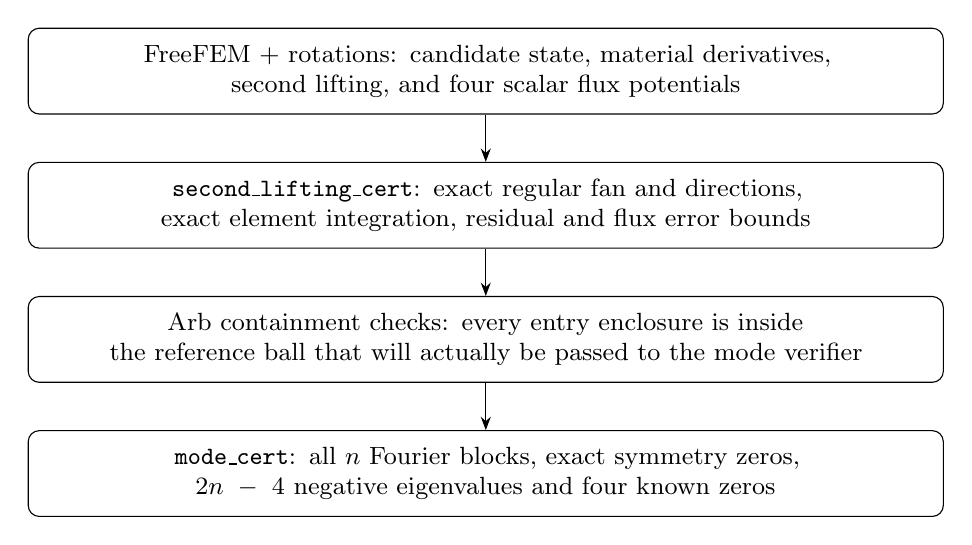
\begin{tikzpicture}[node distance=6mm,
 box/.style={draw,rounded corners,align=center,text width=11.2cm,
 inner sep=6pt,font=\small},>=Stealth]
\node[box] (a) {FreeFEM + rotations: candidate state, material derivatives,\\
 second lifting, and four scalar flux potentials};
\node[box,below=of a] (b) {\texttt{second\_lifting\_cert}: exact regular fan and directions,\\
 exact element integration, residual and flux error bounds};
\node[box,below=of b] (c) {Arb containment checks: every entry enclosure is inside\\
 the reference ball that will actually be passed to the mode verifier};
\node[box,below=of c] (d) {\texttt{mode\_cert}: all $n$ Fourier blocks, exact symmetry zeros,\\
 $2n-4$ negative eigenvalues and four known zeros};
\draw[->] (a)--(b);\draw[->] (b)--(c);\draw[->] (c)--(d);
\end{tikzpicture}
\end{center}

FreeFEM and NumPy propose finite element functions. Their linear solves,
floating geometry, and FFTs need not be exact: the C verifier checks the
geometry and directions, then bounds the errors of the supplied functions.
The mathematical identities, the implementation of the two verifiers, and
FLINT/Arb's arithmetic remain part of the trusted argument. This is a
computer-assisted proof, rather than a proof object checked by a formal
proof assistant.

The current source root is \path{MaxTorsionValidation/}. The accompanying
\path{source_index.md} gives function locations, and \path{sources.json}
records the hashes of the files used for these notes. Descriptions below
refer to that snapshot, so a reader can distinguish it from sources saved
inside an older computation archive.

\section{The finite element data entering one entry check}
Write $\vartheta=2\pi/n$. Subdivide each coarse fan triangle
\[
 T_j=\operatorname{conv}\{0,(\cos j\vartheta,\sin j\vartheta),
                  (\cos((j+1)\vartheta),\sin((j+1)\vartheta))\}
\]
uniformly with $m$ segments on each side. Then
\[
 \#\text{triangles}=nm^2,\qquad
 \#\text{nodes}=1+\frac{nm(m+1)}2,\qquad
 \#\text{boundary nodes}=nm.
\]
Every fine triangle is contained in one coarse sector. Thus the gradients
of the fan extensions and the pullback coefficients are constant on each
fine triangle. This fitted structure is used both in the regularity-based
rate discussion and in the exact coefficient reconstruction.

An export starts with
\begin{lstlisting}
TORSION_SECOND_V2 n m k qa qp ra rp nv nt
\end{lstlisting}
Here $k$ is the Fourier index; \code{qa}, \code{ra} select radial ($0$) or
tangential ($1$) directions, and \code{qp}, \code{rp} select cosine ($0$)
or sine ($1$). The final two integers are the node and triangle counts.
Next come the node coordinates, the three node indices of each triangle,
and twelve nodal arrays, in this order:
\begin{lstlisting}
qx qy rx ry u uq ur zh psi0 psiq psir psiz
\end{lstlisting}
The first four arrays are components of the fan extensions
$\theta_q,\theta_r$. The next four specify conforming candidates for the
state, two first material derivatives, and the second lifting. The final
four specify continuous piecewise affine scalar potentials whose curls
are used in the equilibrated fluxes. An array named \code{u} is therefore
a computed candidate, not the exact torsion solution.

For a nonzero index other than the even Nyquist index, the normalized
real directions are
\begin{align*}
 r^c_{k,j}&=\sqrt{2/n}\cos(kj\vartheta)
                    (\cos j\vartheta,\sin j\vartheta),
                    &&\text{radial, cosine},\\
 t^c_{k,j}&=\sqrt{2/n}\cos(kj\vartheta)
                    (-\sin j\vartheta,\cos j\vartheta),
                    &&\text{tangential, cosine},\\
 t^s_{k,j}&=\sqrt{2/n}\sin(kj\vartheta)
                    (-\sin j\vartheta,\cos j\vartheta),
                    &&\text{tangential, sine}.
\end{align*}
Using the Fourier convention of Lecture 1, the four requested entries are
the following real Hessian pairings:
\begin{center}
\begin{tabular}{@{}llll@{}}
\toprule
Entry name & $q$ & $r$ & Exact value of $D^2\F[q,r]$\\\midrule
\code{rr} & $r_k^c$ & $r_k^c$ & $\alpha_k$\\
\code{tt} & $t_k^c$ & $t_k^c$ & $\beta_k$\\
\code{rt_re} & $r_k^c$ & $t_k^c$ & $\operatorname{Re}(B_k)_{12}=0$\\
\code{rt_im} & $r_k^c$ & $t_k^s$ & $\operatorname{Im}(B_k)_{12}=\gamma_k$\\
\bottomrule
\end{tabular}
\end{center}
For $n$ even and $k=n/2$, replace
$\sqrt{2/n}$ by $1/\sqrt n$ and omit the zero sine direction. Only the two
diagonal pairings are then needed.

\section{Arb arithmetic: enclosures rather than rounded answers}
An Arb real ball represents a midpoint with a rigorous absolute error
radius. Arithmetic propagates enclosures; increasing the precision
reduces rounding error but does not remove finite element error.
The maintained driver uses 192 bits in both verification stages.
The relevant documented operations are: \code{arb_set_str} for decimal
input, \code{arb_add_error} for enlarging a radius,
\code{arb_contains} for containment, and \code{arb_is_negative} for strict
negativity of the whole ball \cite{FLINTArbDocs}.

In particular, a negative midpoint is insufficient. If an enclosure is
$[-3\cdot10^{-5},10^{-6}]$, its sign is unresolved. Similarly, printed
digits are not the internal ball. The driver may use printed output to
propose a convenient radius, but the entry verifier must subsequently
prove that the exact reference ball contains its internal enclosure.

The code uses \code{arb_sqrtpos} only for expressions mathematically
known to be nonnegative, such as sums of squares. Intersecting their
enclosure with the nonnegative half-line is justified by that identity;
it would not justify taking a square root of an arbitrary uncertain input.
The input readers reject nonfinite numbers before they are used in the
certificate.

\section{The entry verifier, function by function}
\label{l3:entryfunctions}
Open \path{MaxTorsionValidation/flint/second_lifting_cert.c}.
The program does not solve a large interval linear system. It integrates
the supplied piecewise affine fields and evaluates the error inequalities
of Lecture 2. Its functions fall into four short groups, followed by the
main calculation.

\subsection{Reading a finite conforming mesh}
\paragraph{\code{die}.}
Print an explanation and exit with status $2$. A failed input assertion
is an error, not a certificate with a large radius.

\paragraph{\code{cmp_edge} and \code{cmp_tri_key}.}
Compare sorted vertex pairs and triples lexicographically. Sorting makes
edge multiplicities and duplicate triangles detectable independently of
their order in the exported file.

\paragraph{\code{dsu_root} and \code{dsu_join}.}
Maintain connected components using a disjoint-set data structure, with
path compression. They supply the connectivity part of the mesh check.

\paragraph{\code{certify_mesh_topology}.}
Check valid and distinct triangle vertices, reject duplicate triangles,
require all nodes to be used and connected, count edges with one or two
incident triangles, and check the boundary degrees, boundary count, and
Euler relation. In strict mode the node and triangle counts must equal
the regular-fan formulas above. The function returns the boundary mask.
These combinatorial conditions are necessary; the later equality with
the complete canonical triangulation establishes the particular mesh
required by the proof.

\paragraph{\code{read_ball} and \code{read_field}.}
Read a finite decimal as an Arb ball and optionally enlarge it by a
specified radius; repeat for a nodal array. Geometry and direction
candidates are initially given radii $10^{-13}$. PDE and potential
coefficients are read with no additional modelling radius: the decimal
coefficients define the candidate finite element function, with conversion
rounding enclosed by Arb. Truncation and nonfinite data are rejected.

\paragraph{\code{assemble_triangle_geometry}.}
Form the signed determinant of the two triangle edge vectors, prove it
does not contain zero, and compute the area and the gradients of the three
barycentric basis functions. The signed determinant is used for gradients;
its absolute value is used for area. Geometry is assembled again after
the exact regular coordinates have replaced the candidate coordinates.

\subsection{Proving the exact regular fan and the directions}
\paragraph{\code{canonical_gid}.}
Give each lattice node of the regular fan a single integer index. The
centre has one index; nodes on shared rays have the same index when
described from either neighboring sector. This is how the program avoids
counting a shared ray twice.

\paragraph{\code{canonical_tri_key}.}
Sort the three canonical node indices of a triangle. This removes an
irrelevant orientation or input-order choice when comparing triangulations.

\paragraph{\code{validate_regular_inputs}.}
Reconstruct the exact node set
\[
 x=\frac{s}{m}(\cos j\vartheta,\sin j\vartheta)
   +\frac{t}{m}(\cos((j+1)\vartheta),\sin((j+1)\vartheta)),
 \qquad s,t\geq0,\quad s+t\leq m.
\]
The integer pair $(s,t)$ is a lattice address, not a new angle notation.
Floating calculations nominate an address; Arb then proves that the
candidate coordinate balls contain the trigonometric coordinates of that
address. The assignment must be a bijection. The boundary mask must agree
with the canonical boundary, and the sorted list of triangles must equal
the full canonical list, not merely have the correct cardinality.

The function also reconstructs the normalized Fourier directions at each
node and proves their containment in the exported direction balls.
It finally replaces geometry and direction arrays by these analytic
enclosures. Each triangle has exact area $\sin\vartheta/(2m^2)$ and the
total area is $n\sin\vartheta/2$. Consequently the $10^{-13}$ input radii
serve to identify the intended exact data; they do not certify an arbitrary
perturbation of the polygon or enter as a shape uncertainty.

\subsection{Exact element integration and coefficient bounds}
\paragraph{\code{gradient}.}
For a nodal scalar field $v$, compute
$\nabla v|_T=\sum_{i=0}^2v_i\nabla\lambda_i$. It is constant on a
triangle, so no numerical quadrature is required.

\paragraph{\code{affine_integral}.}
Use $\int_Tv=|T|(v_0+v_1+v_2)/3$.

\paragraph{\code{add_affine_square}.}
Add the exact integral
\begin{equation}
 \int_Tv^2=\frac{|T|}{6}
 (v_0^2+v_1^2+v_2^2+v_0v_1+v_0v_2+v_1v_2).
 \label{l3:mass}
\end{equation}
This is the usual consistent $P_1$ mass matrix. As a quick check,
$v_0=v_1=v_2=1$ gives $|T|$. Applied separately to the two components of
an affine flux mismatch, it gives its squared $L^2$ norm exactly, with
only interval arithmetic rounding to enclose.

\paragraph{\code{symmetric_norm}.}
For a real symmetric matrix with entries $x,y,z$, compute its operator norm
from
\[
 \left\|\begin{pmatrix}x&y\\y&z\end{pmatrix}\right\|_2
   =\frac{|x+z|+\sqrt{(x-z)^2+4y^2}}2.
\]
Taking a maximum over triangles supplies the constants
$C_q=\|\mathbb A_q\|_{L^\infty}$, $C_r$, and
$C_{qr}=\|\mathbb A_{qr}\|_{L^\infty}$ used in Lecture 2.

\paragraph{\code{coefficients}.}
Differentiate the planar pullback coefficient
\[
 \mathbb A(s,t)=\det(\Id+sD\theta_q+tD\theta_r)
 (\Id+sD\theta_q+tD\theta_r)^{-1}
 (\Id+sD\theta_q+tD\theta_r)^{-T}.
\]
The function returns $\mathbb A_q,\mathbb A_r,\mathbb A_{qr}$ and
the mixed determinant derivative
\[
 (\operatorname{div}\theta_q)(\operatorname{div}\theta_r)
                          -\tr(D\theta_qD\theta_r).
\]
The first matrix derivative is
$\mathbb A_q=(\operatorname{div}\theta_q)\Id-D\theta_q-D\theta_q^T$.
To read the second derivative without an extra chain of aliases, expand it
as
\begin{align*}
 \mathbb A_{qr}={}&
 \bigl((\operatorname{div}\theta_q)(\operatorname{div}\theta_r)
                       -\tr(D\theta_qD\theta_r)\bigr)\Id\\
 &-(\operatorname{div}\theta_q)(D\theta_r+D\theta_r^T)
  -(\operatorname{div}\theta_r)(D\theta_q+D\theta_q^T)\\
 &+D\theta_qD\theta_r+D\theta_rD\theta_q
  +D\theta_q^TD\theta_r^T+D\theta_r^TD\theta_q^T\\
 &+D\theta_qD\theta_r^T+D\theta_rD\theta_q^T.
\end{align*}
The source stores each symmetric matrix in three entries. Its temporary
four-entry arrays named \code{Q} and \code{R} are simply the row-major
Jacobians $D\theta_q,D\theta_r$; no additional mathematical quantities
are needed to understand them.

\paragraph{\code{state_error}.}
Compute
\[
 \Phi_0=\|-x/2+\curl\widetilde\psi_0-\nabla\widetilde u\|_{L^2(P_n)},
 \qquad \curl\psi=(\partial_y\psi,-\partial_x\psi).
\]
The flux has divergence $-1$. Continuity of the scalar potential ensures
the required normal continuity of its curl. Thus $\Phi_0$ bounds the
state energy error even if the auxiliary fit for $\widetilde\psi_0$ is
inexact.

\subsection{Residuals, reference values, and the main calculation}
\paragraph{\code{interior_residual_norm}.}
Take the Euclidean norm of a residual array on the interior nodes only.
The basis of $V_h\subset H^1_0(P_n)$ has no boundary degrees of freedom.
Including the boundary rows of the unconstrained stiffness matrix would
therefore compute the wrong algebraic residual for this problem.

\paragraph{\code{read_mode_reference}.}
Read the requested component of a \code{MODE_DATA} record: \code{rr},
\code{tt}, \code{rt_re}, or \code{rt_im}. These correspond respectively
to the two diagonal entries and the real and imaginary parts of the
upper-right entry. The entry pass checks the requested index and its
conjugate; the final mode pass checks uniqueness and completeness of all
Fourier records.

\paragraph{\code{main}: assertions before the triangle loop.}
Require exactly one of \code{--check-regular-inputs} and
\code{--diagnostic-nonstrict}. Reference certification requires the strict
choice, the reference file, the entry name, and the proposed maximum
radius. Validate dimensions, metadata, and radii; read the export; reject
trailing data. Set the four Dirichlet candidate fields to exact zero on
the certified boundary. The scalar flux potentials have no Dirichlet
condition. Then validate and reconstruct the exact regular inputs.

\paragraph{\code{main}: the triangle loop.}
Accumulate the area, $\int\widetilde u$, the second area variation, the
raw Hessian centre, the three coefficient norm bounds, the four residual
vectors, the node patch areas, and the three remaining squared flux
mismatches. The state mismatch was already evaluated by
\code{state_error}. Each calculation uses constant gradients and
\eqref{l3:mass}; there is no quadrature remainder to estimate.

The mathematical residual convention is
$\rho=\text{right side}-\text{matrix}\times\text{candidate}$.
The C arrays \code{res0}, \code{resq}, \code{resr}, \code{resz}
store its \emph{negative}. Norms do not change, but the sign matters when
correcting the centre.

\paragraph{\code{main}: algebraic errors.}
The polygon lies in $(-1,1)^2$, so domain monotonicity gives
$\lambda_1(P_n)\geq\pi^2/2$. The local mass matrix gives, for the
interior-node stiffness matrix $K_h$,
\[
 K_h\succeq\alpha\Id,\qquad
 \alpha=\frac{\pi^2}{24}
       \min_{i\ \mathrm{interior}}\sum_{T\ni i}|T|>0.
\]
Thus the dual norm of a residual restricted to $V_h$ is bounded by its
Euclidean coefficient norm divided by $\sqrt\alpha$. The first-derivative
algebraic bounds also contain the state error multiplied by $C_q$ or
$C_r$, because the right sides depend on the state candidate.

The corrected centres are those derived in Lecture 2:
\[
 \widetilde C_{\rm corr}
  =\widetilde C+\rho_r(\widetilde u_q)+\rho_0(\widetilde z),
 \qquad
 \widetilde J_{\rm corr}
  =\int_P\widetilde u-\tfrac12\int_P|\nabla\widetilde u|^2.
\]
In the C loop, adding $\rho_r(\widetilde u_q)$ means subtracting
\code{resr} dotted with \code{uq}. The remaining algebraic error in the
Hessian centre is quadratic in the relevant energy errors.

\paragraph{\code{main}: the final entry enclosure.}
Let $\widehat\delta_0,\widehat\delta_q,\widehat\delta_r$ and
$\widehat\eta_{qr}$ denote the computed upper bounds for the state,
first-derivative, and second-lifting Galerkin errors, and let
$E_{\rm alg}$ bound the corrected discrete-centre error. These are the
quantities of Lecture 2, not new error definitions. For the nonzero
Fourier pairings the first area variations vanish. The program evaluates
\begin{align*}
 \widetilde F_{qr}
  &=\frac{\widetilde C_{\rm corr}}{A^2}
        -\frac{2\widetilde J_{\rm corr}A_{qr}}{A^3},\\
 R_F&=\frac{\widehat\delta_q\widehat\delta_r
       +\tfrac12 C_{qr}\widehat\delta_0^2
       +\widehat\delta_0\widehat\eta_{qr}+E_{\rm alg}}{A^2}
       +\frac{|A_{qr}|}{A^3}
                    (\widehat\delta_0^2+\epsilon_0^2).
\end{align*}
Here $A=|P_n|$, $A_{qr}=D^2A[q,r]$, and $\epsilon_0$ bounds the state
algebraic energy error. It enlarges the ball for $\widetilde F_{qr}$ by
$R_F$. Its output separates \code{F_hessian_continuous_error<=} from
\code{F_hessian_algebraic_error<=}, making the source of a large radius
visible.

\paragraph{\code{main}: the handoff assertion.}
If a reference is supplied, reconstruct its ball using the proposed common
mode radius and prove that it contains the complete entry enclosure.
Repeat at the conjugate mode $n-k$; negate the imaginary entry there.
Only successful containment prints
\begin{lstlisting}
ENTRY_CERTIFIED k=... conjugate_k=... entry=... max_radius=...
\end{lstlisting}
The driver checks that all four metadata fields match its request. This
second pass closes the gap between a rigorously computed internal ball
and the finite decimal data actually sent to the eigenvalue verifier.

\section{The Fourier verifier, function by function}
Open \path{MaxTorsionValidation/flint/mode_cert.c}. Its input consists of
\begin{lstlisting}
MODE_DATA k a d Re(b) Im(b)
\end{lstlisting}
representing $\begin{pmatrix}a&b\\\overline b&d\end{pmatrix}$, and a
radius file with one \code{MODE_RADIUS k radius} line for every index.
The letters in this file format mean the two diagonal entries and the
complex upper-right entry; in Lecture 1 these are $\alpha_k,\beta_k$,
and $i\gamma_k$.

\paragraph{\code{usage}.}
Describe the accepted options and exit with status $2$. A global radius
and a per-mode radius file cannot be used together.

\paragraph{\code{print_ball}.}
Print an enclosure for inspection. The displayed precision does not
replace the precision used in the sign predicates.

\paragraph{\code{main}: input validation.}
Read finite real components and nonnegative radii. With the expected
number of symbols specified, require exactly one mode and one radius
for every $k=0,\ldots,n-1$. Reject missing, duplicate, or out-of-range
indices. These checks prevent a repeated negative mode from standing in
for an untested one.

\paragraph{\code{main}: analytic symmetry information.}
With \code{--exact-regular-similarities}, replace $B_0$ by the exact zero
matrix. At $k=1,n-1$, use the exact translation eigenvalue zero and the
trace for the other eigenvalue. At the even Nyquist index, set the
off-diagonal entries to zero. These are analytic identities from Lecture 1;
they are applicable because the first stage proved that the data correspond
to the regular polygon and its normalized Fourier directions.

\paragraph{\code{main}: eigenvalues and sign counts.}
For the remaining blocks evaluate
\[
 \lambda_\pm=
 \frac{a+d\pm\sqrt{(a-d)^2+4(\operatorname{Re}b)^2
                                  +4(\operatorname{Im}b)^2}}2.
\]
Count an eigenvalue as negative only when its entire Arb ball is strictly
negative. The internal word \code{unresolved} includes the four exact
zeros. In a successful regular-polygon run these are its only members.
An interval proved positive is not counted as unresolved; it also cannot
satisfy the required negative count.

The full driver requires all three counts
\[
 \text{symbols}=n,\qquad \text{negative}=2n-4,
                  \qquad \text{unresolved}=4.
\]
The program exits $0$ when the requested counts hold, $3$ when they fail,
and $2$ on an input error. Its printed \code{MODE_CERTIFIED} marker means
the \emph{requested} counts were satisfied. A standalone invocation that
requests weaker counts does not prove local maximality. Nor does this
program prove the PDE error radii: those must come from the entry checks.

\section{How the rotation-based driver obtains the candidates}
\label{l3:driver}
The optimization concerns the first derivatives. At vertex $0$, the local
radial and tangential directions are $(1,0)$ and $(0,1)$. Solve the torsion
problem and these two material problems. Rotational symmetry gives the
other local vertex derivatives by composing these scalar functions with
the inverse rotation. Weighted sums give the Fourier derivatives.
Thus only three primal state/first-derivative solves are needed per polygon.
The present error estimator still solves a second lifting for each real
Hessian pairing, and it computes auxiliary scalar flux fits. Counting
those as well would give more than three linear solves.

\subsection{The FreeFEM problems}
In \path{freefem/second_variation_lifting_rotations.edp}, the named problem
\code{state} is the torsion Galerkin equation, \code{firstQ} and
\code{firstR} are the two differentiated Galerkin equations, and
\code{lifting} is the discrete second lifting of Lecture 2.
The \code{-make-basis 1} branch solves the first three once at vertex $0$.
The \code{-cached-fields} branch reads the state and the requested first
derivatives from the cache and solves only \code{lifting}.

The named problem \code{fitCurl} minimizes a regularized flux mismatch over
continuous piecewise affine scalar potentials. The added term is
$10^{-12}\int_P\psi_h^2/2$ in the minimized functional: it makes the fit
coercive and fixes the additive constant, while also slightly changing the
nonconstant part of the minimizer. Three such fits accompany the initial basis;
one more accompanies each second lifting. The argument for equilibrium
uses the form of the flux, not successful convergence of this optimization.
The solver tolerance affects sharpness and speed, while the C verifier
evaluates the actual supplied potential.

The separate \path{freefem/torsion_hessian_rotations.edp} assembles a
floating Hessian from the same three-solve principle. It is useful for
inspection and comparisons. Its named problems \code{torsion},
\code{materialX}, and \code{materialY} solve the state and the two
coordinate material equations at vertex zero. The driver option \code{--entry-centers}
avoids needing this additional floating Hessian by taking reference
centres directly from the entry estimates.

\subsection{\code{rotation_cache.py}}
\paragraph{\code{prepare}.}
Read the basis export, check dimensions and finiteness, identify lattice
addresses, construct the node permutation for rotation, and check its
cycles and coordinate consistency. Shared-ray addresses have one canonical
key. Apply the permutation to the two vertex-zero scalar solutions and
their flux potentials, then form Fourier combinations with NumPy's FFT.
For NumPy's negative-exponent convention, cosine weights come from the
real part and positive sine weights from the negative imaginary part.
The normalization is $\sqrt{n/2}$, or $\sqrt n$ for the even Nyquist mode,
when dividing an unnormalized Fourier sum.

The nested function \code{direction} selects the radial/tangential and
cosine/sine combination for one requested field. The cache is only a
candidate-generation device: exact geometric and directional checks,
and residual bounds for the resulting fields, are repeated in C.

\subsection{\code{certificate_build.py}}
\paragraph{\code{build_verifiers}.}
Compile \code{second_lifting_cert} and \code{mode_cert} from the source
copies saved inside the new archive, using a forced build. Return their
private executable paths to the driver and record their hashes. A small
diagnostic records the compiler and FLINT header/runtime versions. Failure
of that diagnostic is recorded as unavailable metadata; the two verifier
builds themselves must succeed. The run therefore does not silently use
a pre-existing executable from a different source version.

\subsection{\code{certify_with_rotations.py}}
\paragraph{\code{run}.}
Execute a subprocess, save its output in a designated log, measure elapsed
time, and raise an error for a nonzero exit status. The final mode step is
handled separately so that an inconclusive certificate can be recorded
normally rather than mistaken for a crashed program.

\paragraph{\code{ball}.}
Read the printed midpoint and radius for a named output using decimal
arithmetic. Its result is used to propose a radius. It has no independent
authority to prove containment.

\paragraph{\code{main}: setup and candidate phase.}
Parse the range of $n$, $m$, worker count, CPU affinity limit, flux-fit
tolerance, and a new archive path. Limit numerical-library threads to one
per process, set the chosen affinity, and run with reduced scheduling
priority. Save a source snapshot and manifest, build the private verifiers,
and create the three-solve rotation cache for each polygon.

The nested function \code{evaluate} generates one second-lifting export,
checks its header against the requested pairing, and runs the entry
verifier in strict mode. From the displayed centre and error ball it
proposes a slightly enlarged decimal radius covering both $k$ and $n-k$.
Four pairings are used for each representative nonzero mode, except the
even Nyquist mode, which needs two.

\paragraph{\code{main}: reference and verification phase.}
Once all centres exist, write \code{modes.txt} once and retain it unchanged
during verification. Take the maximum proposed entry radius for each mode
and its conjugate. The nested function \code{verify} reruns the C entry
verifier with this exact reference file and radius, checks the complete
\code{ENTRY_CERTIFIED} marker, and compresses the checked export.
After all entries pass, run \code{mode_cert} at 192 bits with the required
$n,2n-4,4$ counts. Save \code{RESULT.json}, append \code{results.jsonl},
and stop on an inconclusive polygon if \code{--stop-on-failure} is set.
Finally save archive hashes and a \code{FINISHED} marker.

\paragraph{Reading a run's status.}
The Python driver can exit normally after recording
\code{NOT_CERTIFIED}; this is an expected numerical outcome.
\code{FINISHED} means that the requested sweep or its stopping rule has
finished. To claim success for a particular $n$, inspect its
\code{RESULT.json}: it must say \code{status: CERTIFIED} and
\code{mode_exit_code: 0}, with the corresponding entry logs and final
counts present. A shell exit code alone is insufficient.

\section{Other validation utilities and their precise roles}
The two C programs above are the maintained complete certification path.
The repository also contains smaller verifiers and diagnostic utilities.
Their output should be read according to the narrower assertion each
one actually establishes.

\subsection{\code{residual_cert.c}}
\code{read_arb} parses a scalar. Its \code{main} reads a dense matrix,
right side, candidate vector, and a supplied positive lower bound
$\alpha$; it evaluates the residual and the resulting algebraic error
bound. The assumption that the matrix is symmetric positive definite and
that $\alpha\leq\lambda_{\min}$ is supplied by the caller. Positivity of
the number $\alpha$ alone does not prove that assumption. This utility
does not perform the regular-fan and boundary checks of the main verifier.

\subsection{\code{second_variation_cert.c}}
\code{die} reports invalid input; \code{set_nonnegative} parses and checks
nonnegative bounds. The \code{main} function reads complete records of
two direction indices and five bounds, and evaluates
\[
 \delta_q\delta_r+\tfrac12 C_{qr}\delta_0^2+\delta_0\eta_{qr}.
\]
It checks the arithmetic combination, assuming that the five supplied
bounds have already been proved. It does not establish their PDE meaning.

\subsection{\code{majorant_cert.c}}
\begin{longtable}{@{}p{.34\textwidth}p{.62\textwidth}@{}}
\toprule Function & Role\\\midrule\endhead
\code{die} & Reject an invalid export.\\
\code{read_arb}, \code{read_field} & Read scalar balls and arrays.\\
\code{grad_field} & Compute a $P_1$ gradient on a triangle.\\
\code{add_affine_square} & Integrate a squared affine mismatch.\\
\code{energy_norm} & Integrate a field's squared gradient and take its norm.\\
\code{state_majorant} & Bound the state error by its equilibrated flux mismatch.\\
\code{material_majorant} & Bound a first material error, including propagation of the state error.\\
\code{print_ball} & Display an enclosure.\\
\code{main} & Read candidate data and combine direct state/material majorants into diagnostic bounds.\\
\bottomrule
\end{longtable}
This program is useful for understanding individual majorants and direct
Gram estimates. It does not establish the complete canonical-fan input
contract used by \code{second_lifting_cert}; its output alone is not the
maintained local-maximality certificate.

\subsection{Drivers, summaries, and checks}
\path{freefem/test_extended_certificates.py} follows the same two-stage
certificate structure with per-entry candidate solves instead of a shared
rotation cache. Its \code{run}, \code{ball}, nested \code{evaluate} and
\code{verify}, and \code{main} have the corresponding roles described
above. The original candidate-generating FreeFEM files remain available
for comparisons.

In \path{freefem/summarize_extended_certificates.py}, \code{audit} reads an
archive's metadata, source hashes, entry markers, radii, and mode output;
\code{main} assembles the requested result tables. Table upper endpoints
are rounded outward using decimal arithmetic. This is an audit of records,
not a fresh replay of every finite element export.

The input-rejection tests in \path{flint/test_certificate_inputs.py} and
the rotation comparisons in
\path{freefem/test_torsion_hessian_rotations.py} exercise implementation
properties. Neither a successful comparison with floating output nor a
successful test suite substitutes for the entry enclosures and sign counts
for a particular polygon.

\section{Running a certificate yourself}
The commands below are run from the repository root. They require
FreeFEM, a C compiler with FLINT/Arb development files, Python, and NumPy;
the maintained installation instructions are in
\path{MaxTorsionValidation/README.md}. The archive directory must not
already exist, so each run preserves its own evidence.

For a small first run:
\begin{lstlisting}[language=bash]
python3 MaxTorsionValidation/freefem/certify_with_rotations.py \
  5 5 --m 32 --entry-centers --jobs 6 --cpu-cores 6 \
  --stop-on-failure --archive /tmp/torsion_n5_m32_course
\end{lstlisting}
For the largest successfully archived case:
\begin{lstlisting}[language=bash]
python3 MaxTorsionValidation/freefem/certify_with_rotations.py \
  25 25 --m 128 --entry-centers --jobs 6 --cpu-cores 6 \
  --flux-eps 1e-13 --stop-on-failure \
  --archive /tmp/torsion_n25_m128_course
\end{lstlisting}
To test a range, replace the two positional integers by its first and
last $n$. The stopping option halts after the first failure to certify.
For this project's six-physical-core machine the shown settings use six
workers. More generally, \code{--cpu-cores} selects from OS CPU affinity
indices; it does not discover physical-core topology on another machine.

Inspect a completed run with, for example,
\begin{lstlisting}[language=bash]
cat /tmp/torsion_n25_m128_course/n25/RESULT.json
tail -n 2 /tmp/torsion_n25_m128_course/n25/mode_cert.log
\end{lstlisting}
The expected final counts for $n=25$ are $25$ symbols, $46$ negative
eigenvalues, and four exact similarity zeros. The archive also contains
the reference centres, per-mode radii, compressed entry exports, entry
logs, source snapshot, build metadata, and hashes.

An independent replay of a single entry uses the archived verifier and
the decompressed export, with the same \code{--prec 192}, geometry and
direction radii, strict input option, reference file, entry name, and
\code{--max-radius} as its original command. Running only the final
\code{mode_cert} is a useful replay of the small spectral calculation,
but it does not replay the entry PDE bounds.

\section{What the archived computations establish}
\label{l3:results}
The following tables transcribe the manuscript and the archived table
data. No new certification sweep was run to write these notes. All
eigenvalue values refer to $D^2(J/A^2)$ in the normalized vertex coordinates
of Lecture 1. The listed upper bound is the largest certified upper
endpoint among eigenvalues other than the four similarity zeros. Negative
upper bounds are rounded toward $+\infty$, so the displayed values remain
safe upper bounds.

\begin{center}
\begin{tabular}{@{}rrrr@{}}
\toprule
$n$ & $m$ & Negative / required & Upper bound\\\midrule
3&32&2/2&$-1.00\,10^{-2}$\\
4&32&4/4&$-6.20\,10^{-3}$\\
5&32&6/6&$-3.10\,10^{-3}$\\
6&32&8/8&$-1.70\,10^{-3}$\\
7&32&10/10&$-9.80\,10^{-4}$\\
8&32&12/12&$-5.90\,10^{-4}$\\
9&32&14/14&$-3.60\,10^{-4}$\\
10&32&16/16&$-2.20\,10^{-4}$\\
\bottomrule
\end{tabular}
\end{center}
The $n=3,4$ cases are also known analytically. The computations extend the
local-maximality result through $n=25$. Four similarity zeros accompany
every successful row; they are known exactly from invariance, not inferred
from small decimal numbers.

% Generated from archived table JSON; no new computations.

\subsection*{The $m=64$ computations}
\begin{center}\small
\begin{tabular}{@{}rrrrl@{}}
\toprule
$n$ & Triangles & Negative / required & Upper bound & Outcome\\\midrule
11 & 45056 & 18 / 18 & $-2.11\,10^{-4}$ & certified\\
12 & 49152 & 20 / 20 & $-1.50\,10^{-4}$ & certified\\
13 & 53248 & 22 / 22 & $-1.08\,10^{-4}$ & certified\\
14 & 57344 & 24 / 24 & $-7.99\,10^{-5}$ & certified\\
15 & 61440 & 26 / 26 & $-5.97\,10^{-5}$ & certified\\
16 & 65536 & 28 / 28 & $-4.51\,10^{-5}$ & certified\\
17 & 69632 & 30 / 30 & $-3.44\,10^{-5}$ & certified\\
18 & 73728 & 32 / 32 & $-2.64\,10^{-5}$ & certified\\
19 & 77824 & 30 / 34 & $1.35\,10^{-5}$ & inconclusive\\
20 & 81920 & 28 / 36 & $1.69\,10^{-4}$ & inconclusive\\
\bottomrule
\end{tabular}\end{center}

\subsection*{The $m=128$ computations}
\begin{center}\small
\begin{tabular}{@{}rrrrrl@{}}
\toprule
$n$ & Triangles & Negative / required & Upper bound & Minutes & Outcome\\\midrule
19 & 311296 & 34 / 34 & $-2.73\,10^{-5}$ & 15.7 & certified\\
20 & 327680 & 36 / 36 & $-2.22\,10^{-5}$ & 18.0 & certified\\
21 & 344064 & 38 / 38 & $-1.81\,10^{-5}$ & 20.8 & certified\\
22 & 360448 & 40 / 40 & $-1.49\,10^{-5}$ & 13.5 & certified\\
23 & 376832 & 42 / 42 & $-1.24\,10^{-5}$ & 15.8 & certified\\
24 & 393216 & 44 / 44 & $-1.03\,10^{-5}$ & 19.4 & certified\\
25 & 409600 & 46 / 46 & $-8.71\,10^{-6}$ & 17.7 & certified\\
\bottomrule
\end{tabular}\end{center}


At $m=64$, the archived checks succeed through $n=18$ and are inconclusive
for $n=19,20$. A positive upper endpoint in those rows does not prove a
positive eigenvalue. It means the enclosure is too wide to establish all
the desired negative signs. Refinement to $m=128$ succeeds for every tested
$n=19,\ldots,25$. These computations neither establish a maximal possible
$n$ at either mesh size nor give a conclusion beyond $n=25$.

\subsection{Time and the meaning of the three-solve optimization}
The recorded $m=128$ run for $n=25$ took $1059.4$ seconds, about
$17.7$ minutes, on the six-physical-core Intel Core i7-9750H machine
(2.60 GHz). It has $409600$ triangles, $206401$ nodes, and $48$ real
entry checks. The full optimized $n=22,\ldots,25$ records total about
$66.4$ minutes; allowing roughly $70$ minutes is a useful estimate on that
machine. The $n=24$ record includes a handoff interval, and the earlier
$n=19,20,21$ runs used a different allocation/workflow, so the timings do
not form a controlled scaling benchmark.

The three initial primal solves do not make the whole proof constant
cost in $n$: there are more modes, more mesh triangles, one second lifting
and one auxiliary flux fit per real pairing, and two Arb entry passes.
This explains why the optimization is substantial while certification
still takes minutes.

\subsection{Where the evidence is stored}
The main archive groups are under \path{MaxTorsionValidation/results/}:
\begin{itemize}
\item \path{review_2026_09_08_certificate_archive}: the $m=32$ chain.
\item \path{extended_m128_fast_n19_onward}: the $m=128$, $n=19,20,21$ records.
\item \path{extended_m128_rotations_n22_n30}: the completed $n=22,23,24$
records; the folder name records an initial range, not results through $30$.
\item \path{extended_m128_rotations_n25}: the separate $n=25$ certificate.
\item \path{extended_m64_table_data.json} and
\path{extended_m128_table_data.json}: the audited table rows and their
per-row log references.
\end{itemize}
The packaging rename from \path{code/} to \path{MaxTorsionValidation/}
preserved historical archives byte for byte. Consequently an old JSON
record can still contain a \path{code/results/...} path; resolve that
prefix to the current source root when locating the file. The packaging
provenance explains this explicitly.

The recorded validity review checked 672 entry-log records, replayed 25
final mode checks, and performed four complete entry replays. Its archive
hash audit covered 2701 files and recorded one historical checksum mismatch
for the compressed $n=21$, $k=6$, radial--radial export. That entry was
freshly recertified at the archived radius; the original checksum record
was retained and the replay documented in
\path{validity_review_20260909/n21-replay-provenance.json}.
This is the precise scope of that review: it was not a fresh recomputation
of all 672 entry exports. Hashes establish correspondence of bytes;
the mathematical conclusion comes from the verification chain applied
to the identified data.

\subsection*{Exercises and audit questions}
\begin{exercise}
An FFT bug changes a cached first derivative. Why can the full chain still
be valid if it reports success?
\end{exercise}
\noindent\emph{Answer.} The cached field is merely a conforming candidate.
The C verifier computes its residual and flux mismatch for the prescribed
exact direction. A poor candidate normally widens the enclosure or causes
failure; it is not assumed to solve the intended PDE.

\begin{exercise}
The entry pass gives an enclosure centred at $c$ with radius $r$. The mode
file stores a decimal $c_0$. Is using radius $r$ around $c_0$ sufficient?
\end{exercise}
\noindent\emph{Answer.} In general no: the difference between $c_0$ and the
entry centre must be covered as well. The second C pass proves containment
of the whole internal enclosure in the ball built from the actual mode
file, and also checks the conjugate entry.

\begin{exercise}
Why are four exact zeros compatible with strict local maximality?
\end{exercise}
\noindent\emph{Answer.} They are precisely the tangent directions to
similarities, along which $J/A^2$ is constant. On a local slice fixing
translation, rotation, and scale, the Hessian is strictly negative definite.

\begin{exercise}
What follows if \code{RESULT.json} says \code{NOT_CERTIFIED} at $m=64$?
\end{exercise}
\noindent\emph{Answer.} This chain at this mesh and these candidates has
not proved the required signs. It supplies no counterexample to local
maximality. The successful $m=128$ checks for $n=19,20$ illustrate the
difference between a failed enclosure test and a false mathematical claim.

\bibliographystyle{abbrv}
\bibliography{references}
\end{document}
